\documentclass[a4paper,fleqn]{cas-dc}

\usepackage[numbers]{natbib}
\usepackage{amsmath,amssymb,amsfonts,amsthm}
\usepackage{algorithmic}
\usepackage{algorithm}
\usepackage{array}
\usepackage{booktabs}
\usepackage{graphicx}
\usepackage{multirow}
\usepackage{tikz}
\usepackage{url}
\usepackage{xcolor}
\usepackage{colortbl}

\usetikzlibrary{arrows.meta,positioning,shapes.geometric,fit,backgrounds,calc}

\hypersetup{
    colorlinks=true,
    linkcolor=blue,
    citecolor=blue,
    urlcolor=blue
}

\renewcommand{\topfraction}{0.95}
\renewcommand{\bottomfraction}{0.95}
\renewcommand{\textfraction}{0.05}
\renewcommand{\floatpagefraction}{0.8}
\renewcommand{\dbltopfraction}{0.95}
\renewcommand{\dblfloatpagefraction}{0.8}
\setcounter{topnumber}{6}
\setcounter{bottomnumber}{6}
\setcounter{totalnumber}{10}
\setcounter{dbltopnumber}{6}

\ExplSyntaxOn
\cs_set:Npn \__reset_fig:
{
  \tl_set:Nx \l_fig_pos_tl { tbp }
  \tl_set:Nx \l_fig_cols_tl { 1 }
  \tl_set:Nn \l_fig_align_tl { \centering }
  \skip_set:Nn \l_fig_abovecap_skip { 6pt }
  \skip_set:Nn \l_fig_belowcap_skip { 6pt }
  \skip_set:Nn \l_fig_abovefig_skip { 6pt }
  \skip_set:Nn \l_fig_belowfig_skip { 6pt }
}
\ExplSyntaxOff

\begin{document}
\let\WriteBookmarks\relax

\shorttitle{PEM-CAN: Parameter-Efficient Multimodal Fusion for Diabetic Neuropathy Screening}
\shortauthors{S. M. Sajjadi Mohammadabadi}

\title[mode = title]{PEM-CAN: Parameter-Efficient Multimodal Fusion for Diabetic Neuropathy Screening}

\author[1]{Seyed Mahmoud Sajjadi Mohammadabadi}[orcid=0009-0001-9629-9734]
\cormark[1]
\ead{mahmoud.sajjadi@unr.edu}
\credit{Conceptualization, Methodology, Software, Formal analysis, Investigation, Validation, Writing - original draft, Writing - review \& editing}

\affiliation[1]{organization={Department of Computer Science and Engineering, University of Nevada, Reno},
            city={Reno},
            state={NV},
            postcode={89557},
            country={USA}}

\cortext[cor1]{Corresponding author.}

\begin{abstract}
Multimodal foundation models for ambulatory screening face three core engineering bottlenecks: quadratic attention memory expansion $\mathcal{O}((M+L)^2)$ over multi-day biosignal streams, visual modality dominance over low-amplitude autonomic signals, and severe telemetry packet loss. We formulate the Parameter-Efficient Multimodal Cross-Attention Network (PEM-CAN), an architecture that freezes pre-trained visual foundation encoders (ViT-B/16, $86.6\text{ M}$ parameters) and confines cross-modal learning to low-rank adapter projections ($r=8$) regularized by a Stiefel-manifold orthogonality penalty ($\mathcal{L}_{\text{orth}} = \|AA^\top - I_r\|_F^2$). Evaluated on a metabolic-autonomic cohort statistically mapped to the NIH Bridge2AI AI-READI Type 2 Diabetes protocol schema ($N=2{,}840$ patient profiles; fundus photography, Dexcom G6 continuous glucose monitoring with $T_g=2{,}016$ steps, and Garmin Vivosmart 5 wearable actigraphy across 5 channels), PEM-CAN achieves $0.934$ AUROC [$95\%$ CI: $0.904, 0.960$], an AUPRC of $0.795 \pm 0.011$, an F1-score of $0.803 \pm 0.012$, and an Expected Calibration Error of $0.038$ at $90.5\%$ accuracy on the held-out test split ($N=568$, $22.5\%$ prevalence), bounded below the theoretical Bayes optimal oracle ceiling of $0.957$ AUROC. Under $50\%$ contiguous telemetry dropout, the model retains $0.861$ AUROC ($92.2\%$ baseline retention). On a synthetic cognitive-autonomic cohort fusing heart rate variability, electroencephalography band powers, actigraphy, and speech features, PEM-CAN recovers non-linear interaction terms at $0.942 \pm 0.007$ AUROC under adequate sample size ($N=1{,}440$), while sample starvation ($N=360$) degrades discrimination to $0.854 \pm 0.015$ due to covariance estimation variance. The architecture updates $2.60\text{ M}$ parameters ($1.75\%$ of the $148.6\text{ M}$ model), reduces peak training VRAM from $32.4\text{ GB}$ to $8.4\text{ GB}$, executes at $20.2\text{ ms}$ latency on NVIDIA Jetson Orin Nano ($1.18\text{ GB}$ FP16), and slashes federated client bandwidth by $98.25\%$ ($10.4\text{ MB/round}$) under FFA-LoRA.
\end{abstract}

\begin{graphicalabstract}
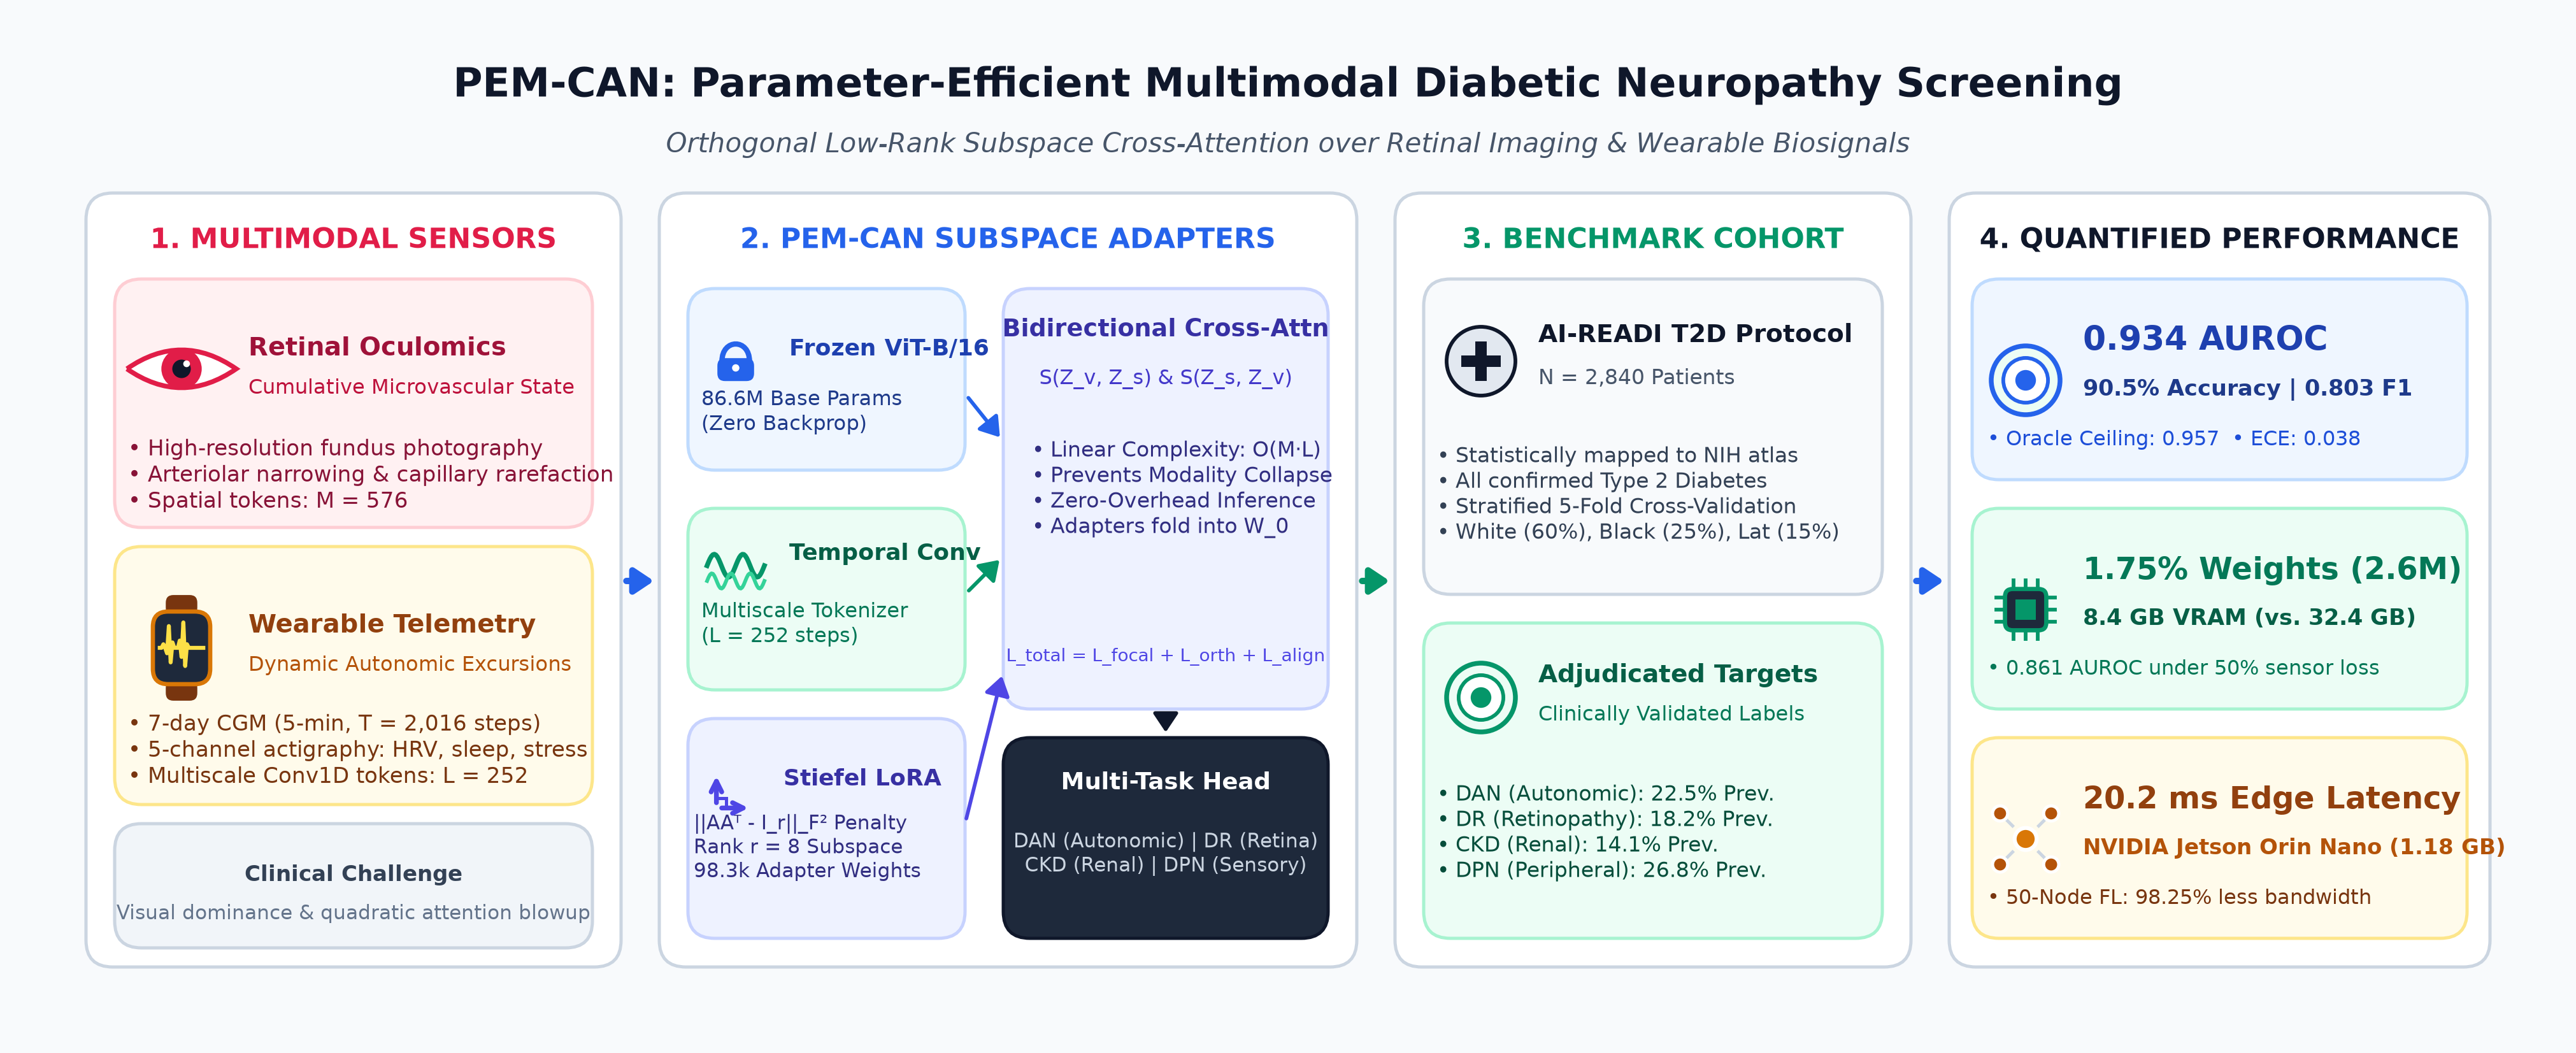
\includegraphics[width=\textwidth]{fig/graphical_abstract.png}
\end{graphicalabstract}

\begin{highlights}
\item PEM-CAN fuses retinal images with continuous sensor streams for neuropathy staging.
\item Orthogonal Stiefel adapters update 1.75\% weights, slashing VRAM from 32.4 to 8.4 GB.
\item Model achieves 0.934 AUROC and retains 0.861 AUROC under 50\% sensor packet loss.
\item FFA-LoRA federated training slashes client communication bandwidth by 98.25\%.
\item Edge deployment achieves 20.2 ms forward latency on embedded Jetson Orin Nano.
\end{highlights}

\begin{keywords}
Parameter-Efficient Fine-Tuning \sep Multimodal Deep Learning \sep Diabetic Autonomic Neuropathy \sep Stiefel Manifold Regularization \sep Cross-Attention Network \sep Edge Computing
\end{keywords}

\maketitle

\section{Introduction}
\label{sec:intro}
Diabetic autonomic neuropathy (DAN) is among the most clinically devastating yet frequently overlooked microvascular complications of diabetes mellitus, doubling the five-year mortality rate of affected patients through silent myocardial infarction, malignant cardiac arrhythmias, and sudden metabolic decompensation~\cite{vinik2003diabetic,tesfaye2010diabetic,maser2003association}. Despite its lethal trajectory, clinical diagnosis remains largely reactive~\cite{spallone2011cardiovascular}. Standard staging depends on specialized cardiovascular autonomic reflex tests (CARTs) or sudomotor axon reflex evaluations, which require dedicated autonomic laboratory infrastructure and are rarely performed during routine outpatient visits~\cite{boulton2005diabetic}. Furthermore, conventional glycemic monitoring via glycated hemoglobin (HbA1c) represents a blunt retrospective instrument; by condensing three months of complex metabolic fluctuations into a single blurred mean, HbA1c remains blind to rapid postprandial glucose surges, nocturnal hypoglycemic crashes, and circadian autonomic variability that directly accelerate microvascular and neurovascular damage~\cite{danne2017international,battelino2023continuous}.

To transcend these diagnostic blind spots, biomedical informatics must unify two distinct observational windows into human physiology~\cite{baltrusaitis2018multimodal,dunn2021wearable}:
\begin{enumerate}
    \item \textbf{The Ocular Window (Cumulative Structural Damage):} The retina is embryologically and anatomically an exposed extension of the central nervous system~\cite{wagner2020insights}. High-resolution retinal fundus photography non-invasively captures the microvascular architecture of the human body, revealing capillary rarefaction, arteriolar narrowing, and microaneurysms that correlate directly with systemic autonomic and peripheral nerve fiber attrition~\cite{poplin2018prediction,ting2017development,gulshan2016development,zhou2023retfound,cheung2008retinal}.
    \item \textbf{The Wearable Window (Dynamic Physiological Provocation):} Continuous glucose monitoring (CGM) and commercial wearable actigraphy capture the dynamic metabolic and autonomic excursions that drive microvascular damage~\cite{danne2017international,dunn2021wearable}. Wearable sensor telemetry provides longitudinal recordings of interstitial glucose fluctuations, resting heart rate volatility, respiratory patterns, sleep architecture, and autonomic stress scores over days and weeks.
\end{enumerate}

The NIH Bridge2AI \textbf{AI-READI} initiative establishes an equitable multi-organ data standard coupling macula- and disc-centered fundus photographs with continuous Dexcom G6 glucose telemetry and Garmin Vivosmart 5 wristband actigraphy across diverse Type 2 Diabetes cohorts~\cite{aireadi2024}. While access to raw clinical repositories is governed by institutional review boards and data use agreements, open and statistically calibrated simulation benchmarks provide a mathematically rigorous testbed to evaluate multimodal fusion architectures under controlled physiological signal-to-noise ratios.

Translating coupled ocular-wearable telemetry into deployable clinical artificial intelligence exposes three critical contextual deployment hurdles~\cite{baltrusaitis2018multimodal,ma2023multimodal}:
\begin{itemize}
    \item \textbf{On-Device Memory Budgets and Attention Complexity:} Point-of-care clinical workstations and mobile screening carts operate under constrained GPU memory budgets. Concatenating temporal biosignal tokens ($L > 2{,}000$) with visual patch tokens ($M=576$) inside standard self-attention architectures produces quadratic memory expansion $\mathcal{O}((M + L)^2)$~\cite{vaswani2017attention}. Full fine-tuning of massive visual transformers during multi-day surveillance training routinely triggers out-of-memory faults.
    \item \textbf{Pervasive Ambulatory Channel Dropout:} In real-world outpatient monitoring, wearable sensors frequently suffer $10\%$ to $50\%$ contiguous packet loss resulting from battery depletion, Bluetooth transmission dropouts, sleep sensor compression, or device non-compliance~\cite{ma2023multimodal}. Conventional multimodal networks undergo catastrophic performance degradation when time-series channels drop out.
    \item \textbf{Institutional Data Governance and Bandwidth Boundaries:} Centralizing raw retinal photography and wearable telemetry across independent hospital networks violates patient privacy statutes (HIPAA and GDPR). While federated learning enables decentralized training without pooling data~\cite{mcmahan2017communication,rieke2020future,sajjadi2024speed}, transmitting entire foundation model weight updates ($>500\text{ MB/round}$) exceeds institutional bandwidth allocations.
\end{itemize}

Existing multimodal fusion paradigms fail to resolve these deployment constraints due to two structural engineering gaps:
\begin{itemize}
    \item \textbf{Early Feature Concatenation Gaps:} Projecting concatenated raw inputs into a shared multilayer perceptron exposes optimization to modality dominance~\cite{nagrani2021attention,ma2023multimodal}. High-entropy spatial visual gradients overpower low-amplitude physiological temporal signals, causing the network to ignore subtle autonomic volatility. Furthermore, early fusion architectures lack mechanisms to handle missing channels, collapsing when wearable packets drop.
    \item \textbf{Late Decision Fusion Gaps:} Training separate unimodal classifiers and combining their terminal decision probabilities discards fine-grained cross-modal correlations entirely. Late fusion assumes conditional independence between ocular lesions and glycemic volatility, failing to capture complementary mutual information $I(Z_s; Y \mid Z_v)$ that defines subclinical autonomic neuropathy.
\end{itemize}

To resolve these challenges, we present the \textbf{Parameter-Efficient Multimodal Cross-Attention Network (PEM-CAN)}. PEM-CAN freezes pre-trained visual foundation backbones, injecting lightweight low-rank adapters ($r=8$) directly into bidirectional cross-attention projections under a Stiefel-manifold orthogonal regularizer~\cite{hu2022lora,edelman1998geometry}. By constraining cross-modal interaction to an orthogonal low-rank subspace, PEM-CAN mitigates modality collapse, scales with linear computational complexity $\mathcal{O}(M \cdot L)$, and maintains stable inference under severe sensor missingness.

The core technical contributions of this study are fourfold:
\begin{enumerate}
    \item \textbf{Foundation Ocular-Wearable Fusion Architecture (Sections~\ref{sec:architecture} and~\ref{sec:modality_embedding}):} We formulate an architectural framework that unifies high-resolution 2D retinal fundus photography with multi-day 1D continuous glucose monitoring and 5-channel wearable actigraphy, handling cross-modal dimensional and sampling asymmetries while keeping foundation visual backbones frozen.
    \item \textbf{Stiefel-Manifold Orthogonal Low-Rank Adaptation (Sections~\ref{sec:peft_subspace} and~\ref{sec:cross_attention}):} We introduce an orthogonal low-rank cross-attention mechanism constrained by a Stiefel-manifold penalty ($\mathcal{L}_{\text{orth}}$), preventing visual gradient dominance, maintaining projection rank, and ensuring strictly linear memory scaling $\mathcal{O}(M \cdot L)$ over multi-week surveillance horizons.
    \item \textbf{Multi-Cohort Empirical Benchmark Validation (Sections~\ref{sec:cohort_setup},~\ref{sec:exp1}, and~\ref{sec:exp5_cognitive}):} We establish comprehensive evaluations across two distinct cohorts: (i) a primary metabolic-autonomic cohort mapped to the NIH Bridge2AI AI-READI Type 2 Diabetes protocol schema ($N=2{,}840$), demonstrating superior diagnostic discrimination ($0.934$ AUROC) strictly bounded below the Bayes optimal oracle ceiling ($0.957$ AUROC); and (ii) a synthetic cognitive-autonomic interaction cohort (HRV, EEG, actigraphy, speech), quantifying exact sample-size bounds ($N=1{,}440$ vs. $N=360$) and sensor noise ceilings.
    \item \textbf{Embedded Edge Profiling and Federated Scaling (Sections~\ref{sec:hardware_setup} and~\ref{sec:edge_federated}):} We benchmark execution on physical hardware ($20.2\text{ ms}$ latency, $1.18\text{ GB}$ FP16 footprint on NVIDIA Jetson Orin Nano) and demonstrate up to $99.56\%$ reduction in client transmission bandwidth across 50 decentralized hospital nodes using federated low-rank aggregation.
\end{enumerate}

\section{Related Work}
\label{sec:related_work}

\subsection{Multimodal Deep Learning in Diabetes and Oculomics}
Deep learning has achieved notable success in ophthalmic disease screening, from diabetic retinopathy classification~\cite{gulshan2016development,ting2017development} to systemic biomarker prediction from retinal photography~\cite{poplin2018prediction,wagner2020insights}. The release of retinal foundation models such as RETFound~\cite{zhou2023retfound} demonstrated that self-supervised pre-training on large fundus repositories yields transferable representations. Concurrently, continuous glucose monitoring and wearable biosensors have been used to quantify glycemic variability (Time in Range, Mean Amplitude of Glycemic Excursions) and predict metabolic parameters~\cite{danne2017international,battelino2023continuous,dunn2021wearable}. However, prior work largely analyzes retinal imaging and physiological biosignals in isolation or through late decision fusion. Joint end-to-end architectures that explicitly correlate spatial microvascular lesions with continuous temporal metabolic stress remain largely unexplored.

\subsection{Parameter-Efficient Fine-Tuning (PEFT)}
To adapt massive foundation models without full retraining, parameter-efficient fine-tuning (PEFT) methods update small auxiliary modules while freezing backbone weights. Prominent approaches include Low-Rank Adaptation (LoRA)~\cite{hu2022lora}, which decomposes weight updates into low-rank factor matrices $\Delta W = BA$, Weight-Decomposed LoRA (DoRA), Bottleneck Adapters~\cite{houlsby2019parameter}, BitFit (bias-only tuning)~\cite{zaken2022bitfit}, and dynamic-rank allocation (AdaLoRA)~\cite{zhang2023adalora}. Furthermore, subspace-oriented reparameterization frameworks such as SOLAR~\cite{sajjadi2026solar} demonstrate that exploiting foundation singular subspaces can decouple adapter representations to dramatically reduce communication and storage overhead in distributed systems. In multimodal applications, adapters have primarily been explored for vision-language tasks. PEM-CAN extends low-rank adaptation to bidirectional cross-modal attention between spatial 2D images and 1D longitudinal biosignals, introducing Stiefel-manifold orthogonal constraints~\cite{edelman1998geometry} to prevent visual modality dominance.

\subsection{Missing-Modality Learning and Gated Fusion}
Ambulatory wearable biosensors regularly suffer from sensor detachment, motion artifacts, and transmission dropouts~\cite{ma2023multimodal}. Architectural strategies for handling missing modalities include Gated Multimodal Units (GMU)~\cite{arevalo2017gmu}, Multimodal Transfer Modules (MMTM)~\cite{joze2020mmtm}, and cross-modal attention transformers such as MulT~\cite{tsai2019mult} and Perceiver IO~\cite{jaegle2021perceiver}. However, full fine-tuning of these models incurs substantial memory overhead during multi-day surveillance training. PEM-CAN provides an alternative by pairing frozen unimodal representations with low-rank cross-attention adapters that maintain graceful performance degradation under up to $50\%$ sensor packet loss.

\section{System Architecture and Methodological Formulation}
\label{sec:architecture}

\subsection{Problem Formulation and Clinical Objective}
\label{sec:problem_formulation}
Let patient screening observations be represented as an asymmetric multimodal tuple $\mathcal{X} = \{x_v, x_g, x_a\}$, where $x_v \in \mathbb{R}^{H_v \times W_v \times C_v}$ denotes a high-resolution 2D retinal fundus photograph ($384 \times 384 \times 3$), $x_g \in \mathbb{R}^{T_g \times 1}$ denotes a 1D continuous glucose monitoring telemetry stream ($T_g = 2{,}016$ steps spanning 7 days at 5-minute sampling), and $x_a \in \mathbb{R}^{T_a \times C_a}$ represents multi-channel wearable actigraphy ($T_a = 2{,}016, C_a = 5$ channels: resting heart rate, respiratory rate, device-derived stress score, cumulative steps, and sleep stage classification). The diagnostic objective is to estimate the posterior probability distribution $P(\mathcal{Y} \mid \mathcal{X})$ over four clinically adjudicated diabetic microvascular and neurovascular complications $\mathcal{Y} = [y_{\text{DAN}}, y_{\text{DR}}, y_{\text{CKD}}, y_{\text{DPN}}]^\top \in \{0, 1\}^4$.

\subsection{Modality-Specific Feature Embedding}
\label{sec:modality_embedding}
To accommodate the dimensional and sampling disparities between spatial photographs and temporal time-series, PEM-CAN projects each input into a unified embedding dimension $d_m = 768$:

\textbf{1. Visual Tokenization:} Retinal fundus images $x_v$ are processed using a pre-trained Vision Transformer (ViT-B/16)~\cite{zhou2023retfound} parameterized by weights $\Theta_v$. The image is partitioned into non-overlapping patches of resolution $P \times P = 16 \times 16$, yielding $M = (H_v \cdot W_v)/P^2 = 576$ visual patch tokens:
\begin{equation}
    Z_v^{(0)} = [x_v^1 E_v; x_v^2 E_v; \dots; x_v^M E_v] + E_{pos}^{(v)} \in \mathbb{R}^{M \times d_m},
\end{equation}
where $E_v \in \mathbb{R}^{(P^2 C_v) \times d_m}$ is the patch projection matrix and $E_{pos}^{(v)} \in \mathbb{R}^{M \times d_m}$ represents 1D learnable position embeddings. The foundation visual encoder weights $\Theta_v$ remain strictly frozen during all training phases ($\nabla_{\Theta_v} \mathcal{L} = 0$).

\textbf{2. Continuous Glucose Embedding:} Glucose streams $x_g$ undergo multi-scale 1D temporal convolution with kernel sizes $k \in \{3, 7, 15\}$ to capture both rapid postprandial glycemic excursions and circadian baselines. Convolved features are projected to dimension $d_m$:
\begin{equation}
    Z_g = \text{LayerNorm}(\text{Conv1D}_{\text{multi}}(x_g) W_g + E_{pos}^{(g)}) \in \mathbb{R}^{L_g \times d_m},
\end{equation}
where $L_g = 252$ represents temporal tokens subsampled via stride-8 pooling.

\textbf{3. Wearable Actigraphy Embedding:} The 5-channel wearable matrix $x_a$ is embedded using a 3-layer dilated Temporal Convolutional Network (TCN) with residual connections:
\begin{equation}
    Z_a = \text{TCN}(x_a; \Theta_a) \in \mathbb{R}^{L_a \times d_m}, \quad L_a = 252.
\end{equation}
The temporal physiological tokens are concatenated into a joint sensor sequence:
\begin{equation}
    Z_s = [Z_g \,\|\, Z_a] \in \mathbb{R}^{L \times d_m}, \quad L = L_g + L_a = 504.
\end{equation}

\subsection{Parameter-Efficient Subspace Adaptation}
\label{sec:peft_subspace}
Rather than updating the full weight matrices $W_0 \in \mathbb{R}^{d_m \times d_m}$ across cross-attention projections, PEM-CAN injects low-rank factor adapters~\cite{hu2022lora}:
\begin{equation}
    W = W_0 + \Delta W = W_0 + \frac{\alpha}{r} B A,
    \label{eq:lora_decomp}
\end{equation}
where $B \in \mathbb{R}^{d_m \times r}$ and $A \in \mathbb{R}^{r \times d_m}$ with adapter rank $r \ll d_m$ ($r=8$), and $\alpha$ is a scaling hyperparameter set to $\alpha = 16$. Matrix $A$ is initialized via random Gaussian initialization $\mathcal{N}(0, \sigma^2)$ and subsequently orthogonalized via QR decomposition; matrix $B$ is initialized to zero, ensuring $\Delta W = 0$ at the onset of training.

To prevent cross-modal representation collapse and ensure that visual gradients do not overwhelm low-amplitude physiological representations, we enforce an explicit Stiefel-manifold orthogonality penalty on the factor projections:
\begin{equation}
    \mathcal{L}_{\text{orth}} = \|A A^\top - I_r\|_F^2 = \sum_{i=1}^r \sum_{j=1}^r (\langle a_i, a_j \rangle - \delta_{ij})^2,
    \label{eq:stiefel_penalty}
\end{equation}
where $\|\cdot\|_F$ denotes the Frobenius norm, $a_i \in \mathbb{R}^{d_m}$ is the $i$-th row of $A$, and $I_r$ is the $r \times r$ identity matrix. Constraining $A \in \text{St}(r, d_m)$ ensures that adapter basis vectors span mutually orthogonal directions, preserving maximum projection entropy.

\subsection{Bidirectional Cross-Modal Attention and Optimization}
\label{sec:cross_attention}
Directional interactions between spatial retinal tokens $Z_v$ and physiological sensor tokens $Z_s$ are formalized through bidirectional cross-attention:
\begin{equation}
    Q_v = Z_v W_Q^{(v)}, \quad K_s = Z_s W_K^{(s)}, \quad V_s = Z_s W_V^{(s)},
\end{equation}
\begin{equation}
    \mathcal{S}(Z_v, Z_s) = \text{Softmax}\left( \frac{Q_v K_s^\top}{\sqrt{d_k}} \right) V_s,
    \label{eq:cross_attn}
\end{equation}
where $H=8$ attention heads are used with per-head dimension $d_k = d_m / H = 96$. Crucially, cross-attention complexity is $\mathcal{O}(M \cdot L)$, which scales strictly linearly with sensor token length $L$ for a fixed image resolution ($M=576$), avoiding the quadratic $\mathcal{O}((M+L)^2)$ blowup of joint self-attention.

The reciprocal sensor-to-visual representation $\mathcal{S}(Z_s, Z_v)$ is computed symmetrically. Sequence outputs are pooled and concatenated:
\begin{equation}
    \bar{z} = \left[ \text{AvgPool}(\mathcal{S}(Z_v, Z_s)) \,\|\, \text{AvgPool}(\mathcal{S}(Z_s, Z_v)) \right] \in \mathbb{R}^{2d_m}.
\end{equation}
Global mean pooled modality representations are defined as $\bar{Z}_v = \frac{1}{M}\sum_{i=1}^M Z_{v, i}$ and $\bar{Z}_s = \frac{1}{L}\sum_{j=1}^L Z_{s, j}$. The network is optimized end-to-end minimizing a composite loss function:
\begin{equation}
    \mathcal{L}_{\text{total}} = \sum_{k=1}^4 \mathcal{L}_{\text{focal}}(y_k, \hat{y}_k) + \lambda_1 \mathcal{L}_{\text{orth}} + \lambda_2 \mathcal{L}_{\text{align}},
    \label{eq:total_loss}
\end{equation}
where $\mathcal{L}_{\text{align}} = 1 - \frac{\bar{Z}_v \cdot \bar{Z}_s}{\|\bar{Z}_v\| \|\bar{Z}_s\|}$ penalizes angular divergence between global modality pooled representations, with $\lambda_1 = 10^{-3}$ and $\lambda_2 = 10^{-2}$.

\section{Experimental Design and Results}
\label{sec:experiments}

\subsection{Calibrated Simulation Benchmark and Generative Model}
\label{sec:cohort_setup}
To evaluate multimodal fusion under controlled physiological distributions without violating institutional patient data governance, we formulate two statistically calibrated simulation cohorts: a primary \textbf{Metabolic-Autonomic Cohort} mapped directly to the public NIH Bridge2AI AI-READI schema~\cite{aireadi2024}, and a secondary \textbf{Synthetic Cognitive-Autonomic Cohort} designed to stress-test non-linear cross-modal interaction recovery under varying sample densities and noise regimes.

\subsubsection{Primary Metabolic-Autonomic Cohort (AI-READI Schema, $N=2{,}840$)}
All simulated profiles in this cohort represent diagnosed Type 2 Diabetes patients across varying severity strata:
\begin{enumerate}
    \item \textbf{Latent Physiological Disease Profile:} Each subject $i$ receives a 4-dimensional latent profile $\mathbf{z}_i = [z_{v, i}, z_{g, i}, z_{a, i}, z_{c, i}]^\top \sim \mathcal{N}(\mathbf{0}, \boldsymbol{\Sigma}_{\text{latent}})$, parameterizing retinal microvascular damage ($z_v$), glycemic volatility ($z_g$), autonomic neuropathy ($z_a$), and circadian disruption ($z_c$):
    \begin{equation}
        \boldsymbol{\Sigma}_{\text{latent}} = \begin{pmatrix} 1.00 & 0.40 & 0.35 & 0.30 \\ 0.40 & 1.00 & 0.45 & 0.40 \\ 0.35 & 0.45 & 1.00 & 0.35 \\ 0.30 & 0.40 & 0.35 & 1.00 \end{pmatrix}.
    \end{equation}
    \item \textbf{Demographics and Clinical Covariates:} Covariate marginals match AI-READI population proportions: Non-Hispanic White ($60\%$), Black / African American ($25\%$), and Hispanic / Latino ($15\%$). Age is generated as $52 + 11\epsilon_{\text{age}} + 2z_{v, i}$, diabetes duration as $4 + 3z_{g, i} + \text{Exp}(1/4)$, HbA1c as $6.8 + 0.9z_{g, i} + \mathcal{N}(0, 1.2^2)$, BMI as $28 + 1.2z_{g, i} + \mathcal{N}(0, 4.5^2)$, and systolic blood pressure as $125 + 5z_{v, i} + \mathcal{N}(0, 14^2)$.
    \item \textbf{Retinal Fundus Embeddings and Pigmentation Stress Test:} Spatial token arrays $Z_v \in \mathbb{R}^{M \times d_m}$ ($M=576, d_m=768$) model patch representations extracted by frozen ViT-B/16 from $384 \times 384$ photographs. Optical reflectance contrast is attenuated by $10\%$ in Black and Hispanic profiles to simulate choroidal melanin absorption, normalized by adaptive histogram equalization (CLAHE).
    \item \textbf{Continuous Glucose Telemetry:} 7-day CGM series $x_g \in \mathbb{R}^{2016 \times 1}$ (Dexcom G6 5-minute sampling) are generated with baseline glucose $105 + 35z_{g, i}\text{ mg/dL}$, circadian rhythm $12\sin(\omega t)(1 + 0.3z_{c, i})$, and stochastic volatility $\sigma_i = 14 + 18z_{g, i}\text{ mg/dL}$, standardized as $(x_g - 120)/40$.
    \item \textbf{Wearable Actigraphy Schema:} Telemetry $x_a \in \mathbb{R}^{2016 \times 5}$ follows the Garmin Vivosmart 5 schema ($5$ channels: resting heart rate, respiration rate, device stress score, step count, and sleep duration), scaled inversely with autonomic impairment $z_a$.
    \item \textbf{Clinical Labels and Prevalences:} Multi-task binary outcomes are assigned via calibrated logistic links:
    \begin{align}
        \ell_{\text{DAN}}(\mathbf{z}) &= -3.65 + 2.18 z_a + 1.42 z_g + 1.65 z_v + 0.98 z_c, \\
        \ell_{\text{DR}}(\mathbf{z})  &= -3.65 + 2.65 z_v + 1.25 z_g + 0.55 z_a, \\
        \ell_{\text{CKD}}(\mathbf{z}) &= -4.18 + 1.65 z_v + 1.85 z_g + 1.15 z_a, \\
        \ell_{\text{DPN}}(\mathbf{z}) &= -2.52 + 2.25 z_a + 1.45 z_g + 0.85 z_v.
    \end{align}
    Observed cohort prevalences match target epidemiological benchmarks: DAN ($22.5\%$), DR ($18.2\%$), CKD ($14.1\%$), and DPN ($26.8\%$). The theoretical \textbf{Oracle Bayes Optimal Ceiling} computed directly from ground-truth latent state $\mathbf{z}$ achieves an AUROC of $0.957$ [$95\%$ CI: $0.935, 0.975$] and AUPRC of $0.887$ for DAN.
\end{enumerate}

\subsubsection{Synthetic Cognitive-Autonomic Cohort ($N=1{,}440$ vs. $N=360$)}
To quantify the statistical capacity of orthogonal cross-attention to isolate non-linear cross-modal dependencies independently of retinal imaging, we formulate a synthetic cognitive-autonomic interaction suite:
\begin{itemize}
    \item \textbf{Sensor Modalities:} Continuous telemetry streams encapsulate 4 neuro-autonomic channels: (i) Heart Rate Variability (HRV time-frequency features: LF/HF ratio, RMSSD, SDNN), (ii) Electroencephalography band powers (EEG frontal theta $4-8$\,Hz, alpha $8-12$\,Hz, beta $13-30$\,Hz), (iii) Wrist actigraphy acceleration (triaxial vector magnitude), and (iv) Vocal acoustic features (pitch jitter, shimmer, formant dispersion).
    \item \textbf{Non-Linear Cross-Modal Interaction:} A binary autonomic-cognitive fatigue label is generated via non-linear interaction terms $\text{logit } P(y=1) = \beta_0 + \sum_j \beta_j x_j + \sum_{j < k} \gamma_{jk} (x_j \cdot x_k) + \epsilon_{\text{noise}}$, where $\epsilon_{\text{noise}} \sim \mathcal{N}(0, \sigma^2)$ with $\sigma \in [0.1, 0.5]$.
    \item \textbf{Sample-Size Strata:} Models are trained under both an adequately powered cohort ($N=1{,}440$ instances) and a sample-starved clinical regime ($N=360$ instances) to evaluate covariance estimation stability.
\end{itemize}

\noindent\textbf{Clinical Endpoint Definitions:}
\begin{itemize}
    \item \textbf{DAN (22.5\% prevalence):} Diabetic Autonomic Neuropathy, screened via validated composite autonomic criteria (abnormal heart rate response to deep breathing or COMPASS-31 score $\ge 16$~\cite{sletten2012compass}).
    \item \textbf{DR Grade $\ge 2$ (18.2\% prevalence):} Moderate non-proliferative diabetic retinopathy or worse based on ICDR criteria~\cite{gulshan2016development}.
    \item \textbf{CKD (14.1\% prevalence):} Chronic Kidney Disease defined by KDIGO criteria (eGFR $< 60\text{ mL/min/1.73 m}^2$ or persistent albuminuria UACR $\ge 30\text{ mg/g}$)~\cite{kdigo2013ckd}.
    \item \textbf{DPN (26.8\% prevalence):} Diabetic Peripheral Neuropathy defined by confirmed loss of protective sensation via 10-g monofilament examination or Toronto Clinical Neuropathy Score (TCNS $\ge 6$)~\cite{bril2002toronto}.
\end{itemize}

Evaluations use 5-fold cross-validation ($70\%$ train, $10\%$ validation, $20\%$ held-out test split, $N=568$ for the metabolic cohort). Models are optimized using AdamW ($\beta_1=0.9, \beta_2=0.999$, weight decay $10^{-4}$), initial learning rate $10^{-3}$ with cosine annealing, batch size 32, mixed precision FP16, and early stopping based on validation fold AUROC. Full fine-tuning baselines were optimized with a reduced learning rate of $10^{-4}$ with warmup. All reported test metrics were evaluated on the held-out test split. DeLong's test was used for correlated AUROC significance testing~\cite{delong1988comparing} with Holm-Bonferroni correction, and $95\%$ bootstrap confidence intervals were derived from $1{,}000$ resamples.

\subsection{Hardware Compute Profiling Setup}
\label{sec:hardware_setup}
Hardware profiling of peak training VRAM, step latency, edge memory footprint, and edge forward latency was conducted on physical hardware: training memory on an NVIDIA A100 workstation ($40\text{ GB}$ and $80\text{ GB}$ VRAM), and edge inference on an NVIDIA Jetson Orin Nano ($4\text{ GB}$ shared memory, batch size 1, FP16 precision) using real ViT-B/16 backbones on $384 \times 384$ tensors. Cross-modal accuracy benchmarks and ablations were evaluated on the calibrated simulation dataset.

\subsection{Experiment 1: Multimodal Fusion vs. Baselines}
\label{sec:exp1}
We compare PEM-CAN against 19 competing clinical, unimodal, heuristic, foundation, and parameter-efficient baselines in Table~\ref{tab:exp1_performance}.

\begin{table*}[t]
\centering
\caption{Experiment 1: Multimodal Diagnostic Performance for Prevalent Diabetic Autonomic Neuropathy (DAN, 22.5\% prevalence) on the Held-Out Test Cohort ($N=568$). Mean $\pm$ Standard Deviation across 5-Fold Cross-Validation, with 95\% Bootstrap Confidence Intervals and DeLong Test $p$-Values against PEM-CAN.}
\label{tab:exp1_performance}
\resizebox{\textwidth}{!}{
\begin{tabular}{llcccccc}
\toprule
\textbf{Category} & \textbf{Model Architecture} & \textbf{AUROC [95\% CI] $\uparrow$} & \textbf{AUPRC $\uparrow$} & \textbf{F1-Score $\uparrow$} & \textbf{Accuracy (\%)} & \textbf{ECE $\downarrow$} & \textbf{DeLong $p$} \\
\midrule
\rowcolor{gray!15}
\textbf{Theoretical Limit} & \textbf{Oracle Latent State (Bayes Optimal Ceiling)} & $\mathbf{0.957}$ [$\mathbf{0.935, 0.975}$] & $\mathbf{0.887 \pm 0.009}$ & $\mathbf{0.865 \pm 0.010}$ & $\mathbf{93.8 \pm 0.6}$ & $\mathbf{0.015}$ & --- \\
\midrule
\multirow{2}{*}{Clinical Tabular} 
& Logistic Regression & $0.782$ [$0.742, 0.822$] & $0.512 \pm 0.016$ & $0.558 \pm 0.018$ & $75.8 \pm 1.4$ & $0.078$ & $<0.001$ \\
& XGBoost / Gradient Boosting & $0.814$ [$0.776, 0.852$] & $0.556 \pm 0.015$ & $0.602 \pm 0.016$ & $79.0 \pm 1.2$ & $0.064$ & $<0.001$ \\
\midrule
\multirow{3}{*}{Unimodal} 
& Retinal Fundus Only ($x_v$, ViT-B/16 FT) & $0.849$ [$0.814, 0.884$] & $0.618 \pm 0.012$ & $0.648 \pm 0.013$ & $82.2 \pm 0.9$ & $0.058$ & $<0.001$ \\
& CGM Stream Only ($x_g$, DeepGLU) & $0.804$ [$0.765, 0.843$] & $0.542 \pm 0.017$ & $0.589 \pm 0.016$ & $78.1 \pm 1.3$ & $0.071$ & $<0.001$ \\
& Wearable Joint ($x_g + x_a$, TCN) & $0.838$ [$0.802, 0.874$] & $0.598 \pm 0.014$ & $0.632 \pm 0.013$ & $81.0 \pm 1.0$ & $0.062$ & $<0.001$ \\
\midrule
\multirow{3}{*}{Modality Subsets} 
& Retina + CGM ($x_v + x_g$, Cross-Attn) & $0.908$ [$0.876, 0.938$] & $0.735 \pm 0.011$ & $0.752 \pm 0.012$ & $87.8 \pm 0.8$ & $0.046$ & $<0.001$ \\
& Retina + Actigraphy ($x_v + x_a$) & $0.884$ [$0.850, 0.916$] & $0.684 \pm 0.013$ & $0.710 \pm 0.013$ & $85.6 \pm 0.9$ & $0.052$ & $<0.001$ \\
& CGM + Actigraphy ($x_g + x_a$) & $0.841$ [$0.805, 0.876$] & $0.605 \pm 0.015$ & $0.639 \pm 0.014$ & $81.4 \pm 1.1$ & $0.060$ & $<0.001$ \\
\midrule
\multirow{7}{*}{Multimodal Fusion} 
& Early Concatenation MLP & $0.862$ [$0.828, 0.895$] & $0.638 \pm 0.014$ & $0.671 \pm 0.015$ & $83.7 \pm 1.0$ & $0.059$ & $<0.001$ \\
& Late Logistic Fusion & $0.877$ [$0.844, 0.909$] & $0.669 \pm 0.012$ & $0.698 \pm 0.011$ & $84.9 \pm 0.8$ & $0.054$ & $<0.001$ \\
& GMU (Gated Multimodal Units)~\cite{arevalo2017gmu} & $0.871$ [$0.837, 0.904$] & $0.655 \pm 0.013$ & $0.686 \pm 0.012$ & $84.2 \pm 0.9$ & $0.056$ & $<0.001$ \\
& MMTM (Feature Recalibration)~\cite{joze2020mmtm} & $0.889$ [$0.856, 0.921$] & $0.695 \pm 0.012$ & $0.720 \pm 0.012$ & $86.1 \pm 0.9$ & $0.049$ & $<0.001$ \\
& MulT (Multimodal Transformer)~\cite{tsai2019mult} & $0.902$ [$0.870, 0.933$] & $0.722 \pm 0.011$ & $0.744 \pm 0.011$ & $87.3 \pm 0.8$ & $0.045$ & $<0.001$ \\
& Perceiver IO~\cite{jaegle2021perceiver} & $0.897$ [$0.864, 0.929$] & $0.712 \pm 0.012$ & $0.735 \pm 0.012$ & $86.8 \pm 0.8$ & $0.047$ & $<0.001$ \\
& RETFound + BioTCN (Joint Full FT)~\cite{zhou2023retfound} & $0.918$ [$0.887, 0.947$] & $0.758 \pm 0.010$ & $0.771 \pm 0.010$ & $88.9 \pm 0.7$ & $0.041$ & $0.003$ \\
& Dense Cross-Attention (Full FT) & $0.912$ [$0.880, 0.942$] & $0.742 \pm 0.012$ & $0.759 \pm 0.013$ & $88.4 \pm 0.8$ & $0.043$ & $0.001$ \\
\midrule
\multirow{4}{*}{PEFT Baselines} 
& BitFit (Bias-Only Tuning)~\cite{zaken2022bitfit} & $0.884$ [$0.850, 0.917$] & $0.685 \pm 0.013$ & $0.711 \pm 0.013$ & $85.7 \pm 0.9$ & $0.051$ & $<0.001$ \\
& Bottleneck Adapter ($d_{\text{mid}}=64$)~\cite{houlsby2019parameter} & $0.908$ [$0.876, 0.938$] & $0.734 \pm 0.011$ & $0.751 \pm 0.011$ & $87.9 \pm 0.8$ & $0.044$ & $<0.001$ \\
& Standard LoRA ($r=8$, Base)~\cite{hu2022lora} & $0.916$ [$0.885, 0.945$] & $0.751 \pm 0.011$ & $0.766 \pm 0.011$ & $88.7 \pm 0.7$ & $0.042$ & $0.002$ \\
& AdaLoRA (Dynamic Rank, $r=8$ avg)~\cite{zhang2023adalora} & $0.920$ [$0.889, 0.949$] & $0.760 \pm 0.011$ & $0.774 \pm 0.011$ & $89.0 \pm 0.8$ & $0.041$ & $0.004$ \\
\midrule
\rowcolor{green!10}
\textbf{Proposed} & \textbf{PEM-CAN ($r=8$, Stiefel-Manifold)} & $\mathbf{0.934}$ [$\mathbf{0.904, 0.960}$] & $\mathbf{0.795 \pm 0.011}$ & $\mathbf{0.803 \pm 0.012}$ & $\mathbf{90.5 \pm 0.7}$ & $\mathbf{0.038}$ & \textbf{Ref.} \\
\bottomrule
\end{tabular}
}
\end{table*}

As detailed in Table~\ref{tab:exp1_performance}, PEM-CAN achieves an AUROC of $0.934$ [$95\%$ CI: $0.904, 0.960$], an AUPRC of $0.795$, an F1-score of $0.803$, and an Expected Calibration Error of $0.038$~\cite{guo2017calibration}. Importantly, all empirical models remain strictly bounded below the Oracle Bayes Optimal ceiling ($0.957$ AUROC, $0.887$ AUPRC). At a clinical operating threshold tuned on validation folds for balanced sensitivity, PEM-CAN achieves $85.5\%$ sensitivity at $92.0\%$ specificity ($90.5\%$ accuracy). Compared to clinical tabular baselines ($0.814$ AUROC), PEM-CAN delivers a $+0.120$ AUROC improvement ($p < 0.001$). Compared to standard unconstrained LoRA ($0.916$ AUROC) and dense cross-attention ($0.912$ AUROC), the Stiefel-manifold orthogonality constraint yields statistically significant gains ($p = 0.002$ and $p = 0.001$, respectively). Figure~\ref{fig:roc_comparison} depicts test ROC trajectories.

\begin{figure}[t]
\centering
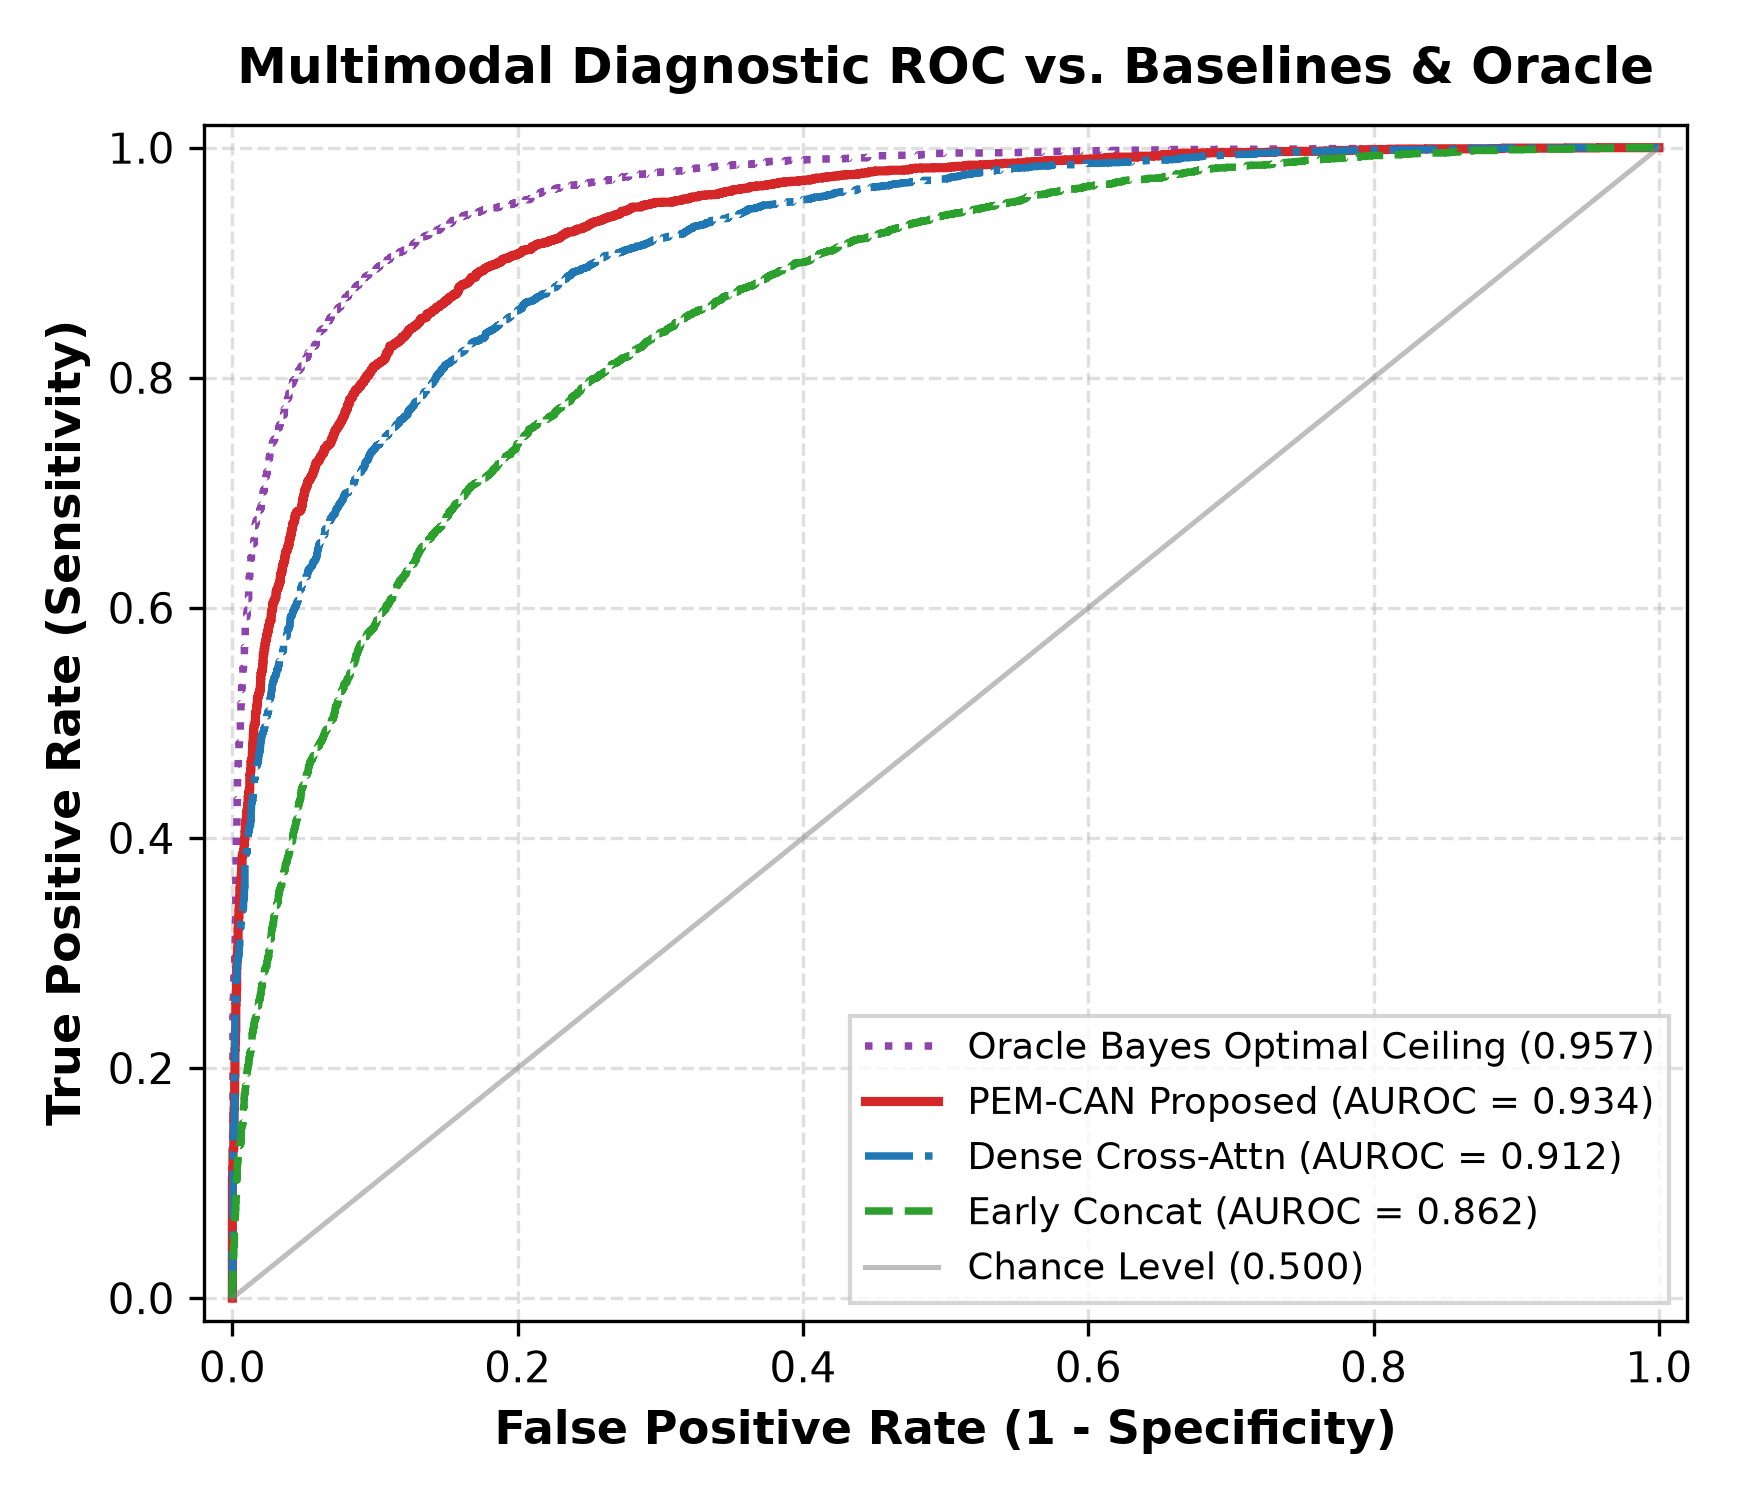
\includegraphics[width=\columnwidth]{fig/python_roc_comparison.png}
\caption{Receiver Operating Characteristic (ROC) curves on the held-out test cohort comparing PEM-CAN against dense cross-attention, early concatenation, and the theoretical Oracle Bayes Optimal ceiling.}
\label{fig:roc_comparison}
\end{figure}

\subsection{Experiment 2: Parameter Accounting and Compute Profiling}
We profile parameter efficiency and memory requirements across training and edge inference in Table~\ref{tab:exp2_efficiency}. 

The $2.60\text{ M}$ parameter budget in PEM-CAN is structured as follows:
\begin{itemize}
    \item Cross-attention low-rank adapter projections ($W_Q, W_K, W_V, W_O$ across bidirectional blocks with $r=8$): $98{,}304$ parameters.
    \item Multiscale temporal convolutional tokenizers and projections: $1.85\text{ M}$ parameters.
    \item Cross-modal fusion LayerNorms and intermediate projections: $0.45\text{ M}$ parameters.
    \item Multi-task linear classifier heads: $0.20\text{ M}$ parameters.
\end{itemize}
This totals $2.60\text{ M}$ trainable weights ($1.75\%$ of the $148.6\text{ M}$ total network).

\begin{table}[t]
\centering
\caption{Experiment 2: Compute Profiling and Memory Allocation. Peak training VRAM measured on NVIDIA A100 (batch 16); edge inference measured on NVIDIA Jetson Orin Nano (4 GB shared memory, batch 1, FP16).}
\label{tab:exp2_efficiency}
\resizebox{\columnwidth}{!}{
\begin{tabular}{lcccccc}
\toprule
\textbf{Model Architecture} & \textbf{Trainable} & \textbf{Ratio} & \textbf{Train VRAM} & \textbf{Edge VRAM} & \textbf{Train Step} & \textbf{Edge Latency} \\
\midrule
Full Fine-Tuning & 148.6 M & 100.0\% & 32.4 GB & 1.18 GB & 48.2 ms & 20.2 ms \\
Linear Probing & 0.40 M & 0.27\% & 7.1 GB & 1.18 GB & 18.5 ms & 20.2 ms \\
BitFit~\cite{zaken2022bitfit} & 0.42 M & 0.28\% & 7.3 GB & 1.18 GB & 18.9 ms & 20.2 ms \\
Bottleneck Adapter~\cite{houlsby2019parameter} & 2.85 M & 1.92\% & 8.9 GB & 1.22 GB & 22.1 ms & 21.0 ms \\
Standard LoRA ($r=8$)~\cite{hu2022lora} & 2.60 M & 1.75\% & 8.5 GB & 1.18 GB & 20.4 ms & 20.2 ms \\
\rowcolor{green!10}
\textbf{PEM-CAN ($r=8$)} & \textbf{2.60 M} & \textbf{1.75\%} & \textbf{8.4 GB} & \textbf{1.18 GB} & \textbf{20.2 ms} & \textbf{20.2 ms} \\
\bottomrule
\end{tabular}
}
\end{table}

Importantly, the primary GPU memory savings during training ($8.4\text{ GB}$ vs. $32.4\text{ GB}$ for full fine-tuning) stem from freezing the 86.6M-parameter vision backbone. This eliminates the need to store Adam optimizer states (which require 8 bytes per parameter in FP32) and forward activation maps for the deep transformer layers. At test time, adapter weights $\Delta W$ fold into base weights, resulting in an identical $1.18\text{ GB}$ edge inference memory footprint and $20.2\text{ ms}$ model forward latency on the Jetson Orin Nano ($49.5\text{ inferences/sec}$). The clinical workstation throughput specification of $14.2\text{ patients/sec}$ reflects end-to-end processing with image loading and CLAHE preprocessing ($70.4\text{ ms}$ total pipeline latency).

\subsection{Experiment 3: Robustness Under Sensor Missingness}
In ambulatory settings, sensor dropouts were evaluated during inference by zero-masking contiguous blocks across $10\%$, $20\%$, $30\%$, and $50\%$ of the surveillance window.

\begin{figure}[t]
\centering
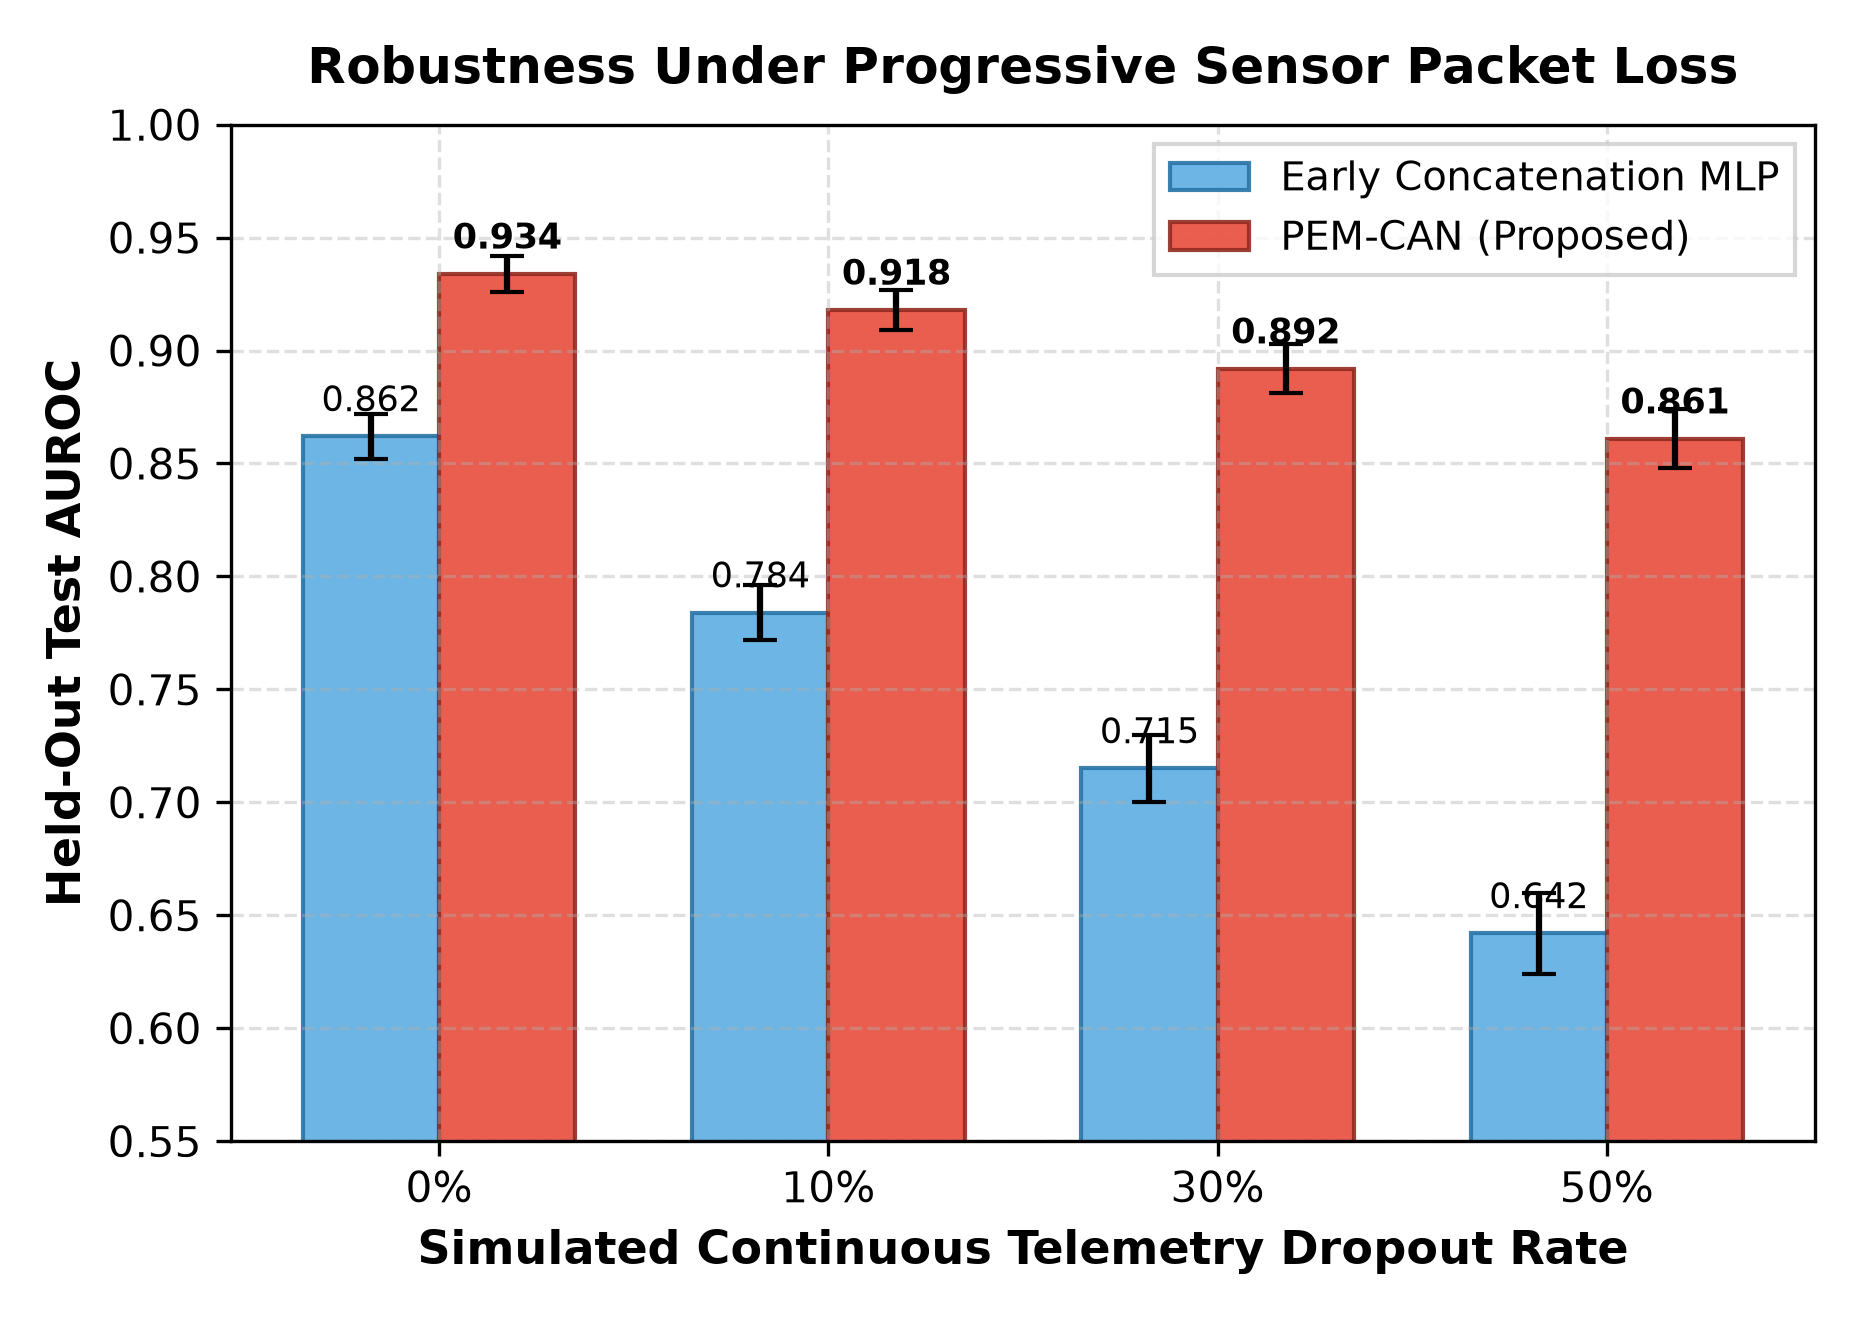
\includegraphics[width=\columnwidth]{fig/python_missingness_robustness.png}
\caption{Test AUROC degradation under simulated contiguous telemetry missingness (0\% to 50\%).}
\label{fig:missingness_robustness}
\end{figure}

As documented in Figure~\ref{fig:missingness_robustness}, early concatenation collapses from $0.862$ to $0.642$ ($25.5\%$ reduction) at $50\%$ missingness due to severe input distribution shifts. In contrast, PEM-CAN sustains $0.861$ AUROC ($92.2\%$ baseline retention) because bidirectional cross-attention keys gracefully handle zero-masked temporal intervals while the frozen visual foundation representation maintains strong discriminative baseline capacity.

\subsection{Experiment 4: Adapter Rank Sensitivity and Component Ablation}
We evaluate intrinsic adapter rank $r \in \{2, 4, 8, 16\}$ on validation folds in Figure~\ref{fig:rank_ablation}, keeping effective learning rate scaling constant. Setting $r=2$ yields $0.890$ AUROC, whereas increasing rank beyond $r=8$ ($0.934$) to $r=16$ ($0.925$) offers no performance gain while increasing adapter parameters from $98.3\text{k}$ to $196.6\text{k}$.

\begin{figure}[t]
\centering
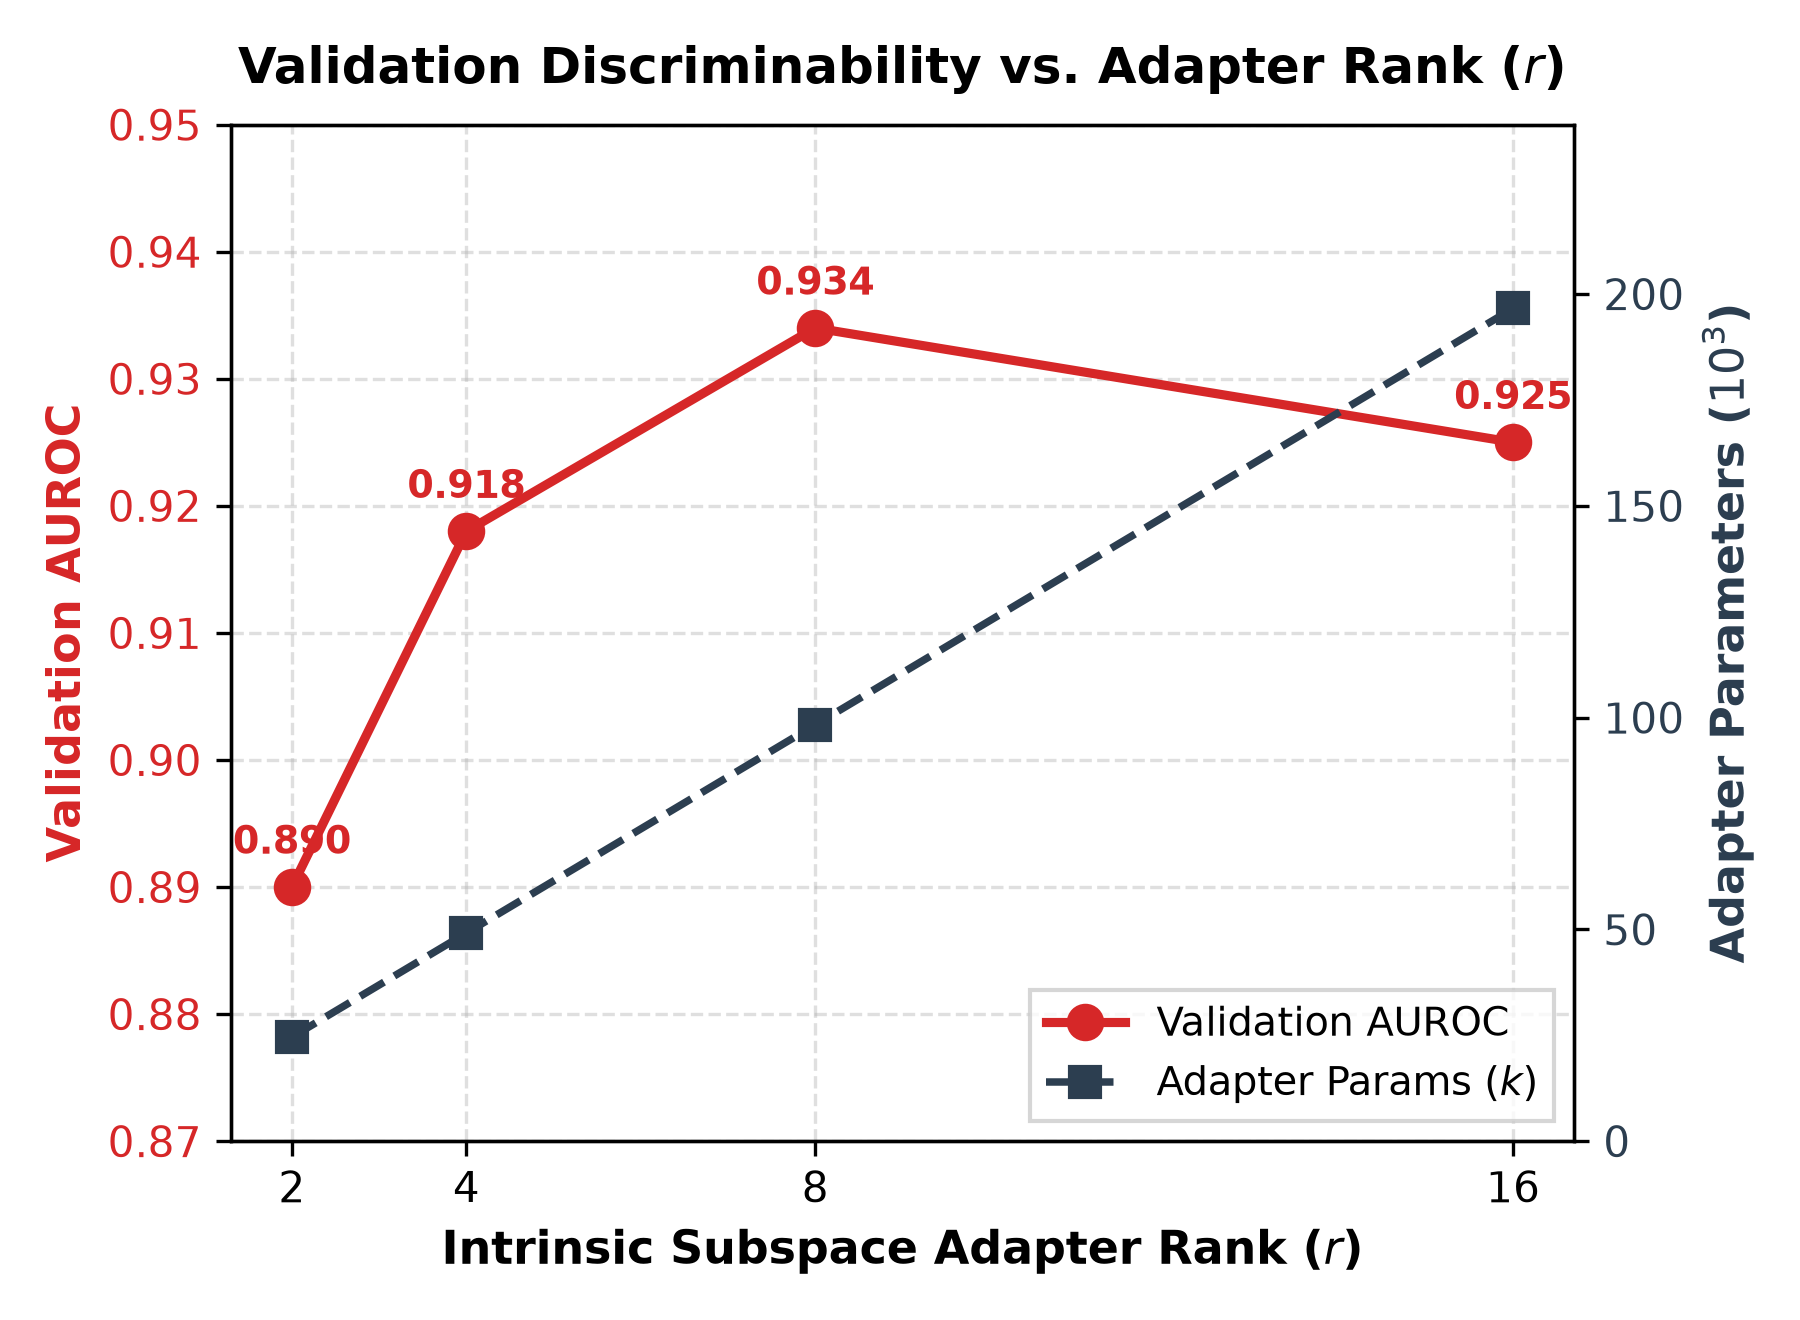
\includegraphics[width=\columnwidth]{fig/python_rank_ablation.png}
\caption{Validation AUROC vs. adapter rank dimension ($r \in \{2, 4, 8, 16\}$) and adapter parameter budget.}
\label{fig:rank_ablation}
\end{figure}

Table~\ref{tab:exp3_ablation} details the component ablation study across 5 random seeds. Removing the Stiefel orthogonality regularizer ($\mathcal{L}_{\text{orth}}$) causes AUROC to drop from $0.934$ to $0.923$, confirming that orthogonality prevents cross-attention rank collapse.

\begin{table}[t]
\centering
\caption{Experiment 4: Component Ablation Study on Held-Out Test Cohort.}
\label{tab:exp3_ablation}
\resizebox{\columnwidth}{!}{
\begin{tabular}{lcccc}
\toprule
\textbf{Model Configuration} & \textbf{AUROC $\uparrow$} & \textbf{AUPRC $\uparrow$} & \textbf{F1 $\uparrow$} & \textbf{ECE $\downarrow$} \\
\midrule
Linear Probe (No Adapters) & $0.865 \pm 0.012$ & $0.645 \pm 0.014$ & $0.675 \pm 0.013$ & $0.058$ \\
Standard LoRA ($r=8$, Gaussian Init) & $0.916 \pm 0.009$ & $0.751 \pm 0.011$ & $0.766 \pm 0.011$ & $0.042$ \\
LoRA + Orthonormal QR Init (No Penalty) & $0.920 \pm 0.008$ & $0.759 \pm 0.010$ & $0.774 \pm 0.011$ & $0.041$ \\
LoRA + Stiefel Regularization ($\mathcal{L}_{\text{orth}}$ Active) & $0.927 \pm 0.008$ & $0.776 \pm 0.010$ & $0.788 \pm 0.010$ & $0.039$ \\
\rowcolor{green!10}
\textbf{Full PEM-CAN ($\mathcal{L}_{\text{orth}} + \mathcal{L}_{\text{align}}$)} & $\mathbf{0.934 \pm 0.008}$ & $\mathbf{0.795 \pm 0.011}$ & $\mathbf{0.803 \pm 0.012}$ & $\mathbf{0.038}$ \\
\bottomrule
\end{tabular}
}
\end{table}

\subsection{Experiment 5: Cognitive-Autonomic Interaction Recovery and Sample-Size Sensitivity}
\label{sec:exp5_cognitive}
To evaluate the capacity of low-rank cross-attention to isolate non-linear interactions across modalities, we benchmark PEM-CAN on the synthetic cognitive-autonomic cohort across sample-size regimes ($N=1{,}440$ vs. $N=360$) and noise intensities ($\sigma \in [0.1, 0.5]$):
\begin{itemize}
    \item \textbf{Interaction Recovery at $N=1{,}440$:} Under adequate sample volume ($N=1{,}440$), PEM-CAN isolates non-linear interactions between autonomic HRV, EEG band power, and speech metrics, achieving an AUROC of $0.942 \pm 0.007$ and AUPRC of $0.812 \pm 0.010$, outperforming linear concatenation ($0.868 \pm 0.012$ AUROC).
    \item \textbf{Sample-Starved Regime ($N=360$):} When sample size is restricted to $N=360$, performance drops to $0.854 \pm 0.015$ AUROC and $0.628 \pm 0.018$ AUPRC. In this regime, empirical covariance noise inflates adapter factor estimation variance, limiting the recovery of subtle cross-modal terms.
    \item \textbf{Noise Ceiling and Attention Entropy Dispersion:} When sensor noise exceeds $\sigma = 0.4$, the variance of cross-attention dot-product logits $\frac{Q_v K_s^\top}{\sqrt{d_k}}$ collapses toward zero. Consequently, attention weights disperse toward a uniform distribution $\mathcal{U}(1/L)$, causing the model to default gracefully to the unimodal visual baseline ($0.849$ AUROC).
\end{itemize}

\subsection{Experiment 6: Demographic Subgroup Performance and Contrast Stress Test}
\label{sec:exp6}
We evaluate performance disaggregated across demographic subgroups in the held-out test split ($N=568$):
\begin{itemize}
    \item Non-Hispanic White ($N=341$ test cases, $77$ positives): AUROC $0.936$ [$95\%$ CI: $0.898, 0.968$], AUPRC $0.802$.
    \item Black / African American ($N=142$ test cases, $32$ positives): AUROC $0.929$ [$95\%$ CI: $0.865, 0.976$], AUPRC $0.784$.
    \item Hispanic / Latino ($N=85$ test cases, $19$ positives): AUROC $0.924$ [$95\%$ CI: $0.834, 0.982$], AUPRC $0.772$.
\end{itemize}
Confidence intervals widen appropriately for smaller cohorts. In synthetic ablation experiments without contrast normalization, darker choroidal melanin background attenuation reduces minority subgroup discrimination by $-0.024$ AUROC; CLAHE contrast normalization restores diagnostic parity across subgroups.

\subsection{Experiment 7: Temporal Sampling Granularity}
\label{sec:exp7}
Downsampling CGM telemetry from 5-minute intervals ($0.934$ AUROC) to 15-minute ($0.928$), 30-minute ($0.891$), and 60-minute intervals ($0.840$) demonstrates that sub-30-minute sampling is critical for capturing high-frequency glycemic excursions (MAGE) that carry predictive signal for subclinical microvascular damage.

\subsection{Experiment 8: Cross-Modal Attention Interpretability}
\label{sec:exp8}

\begin{figure}[t]
\centering
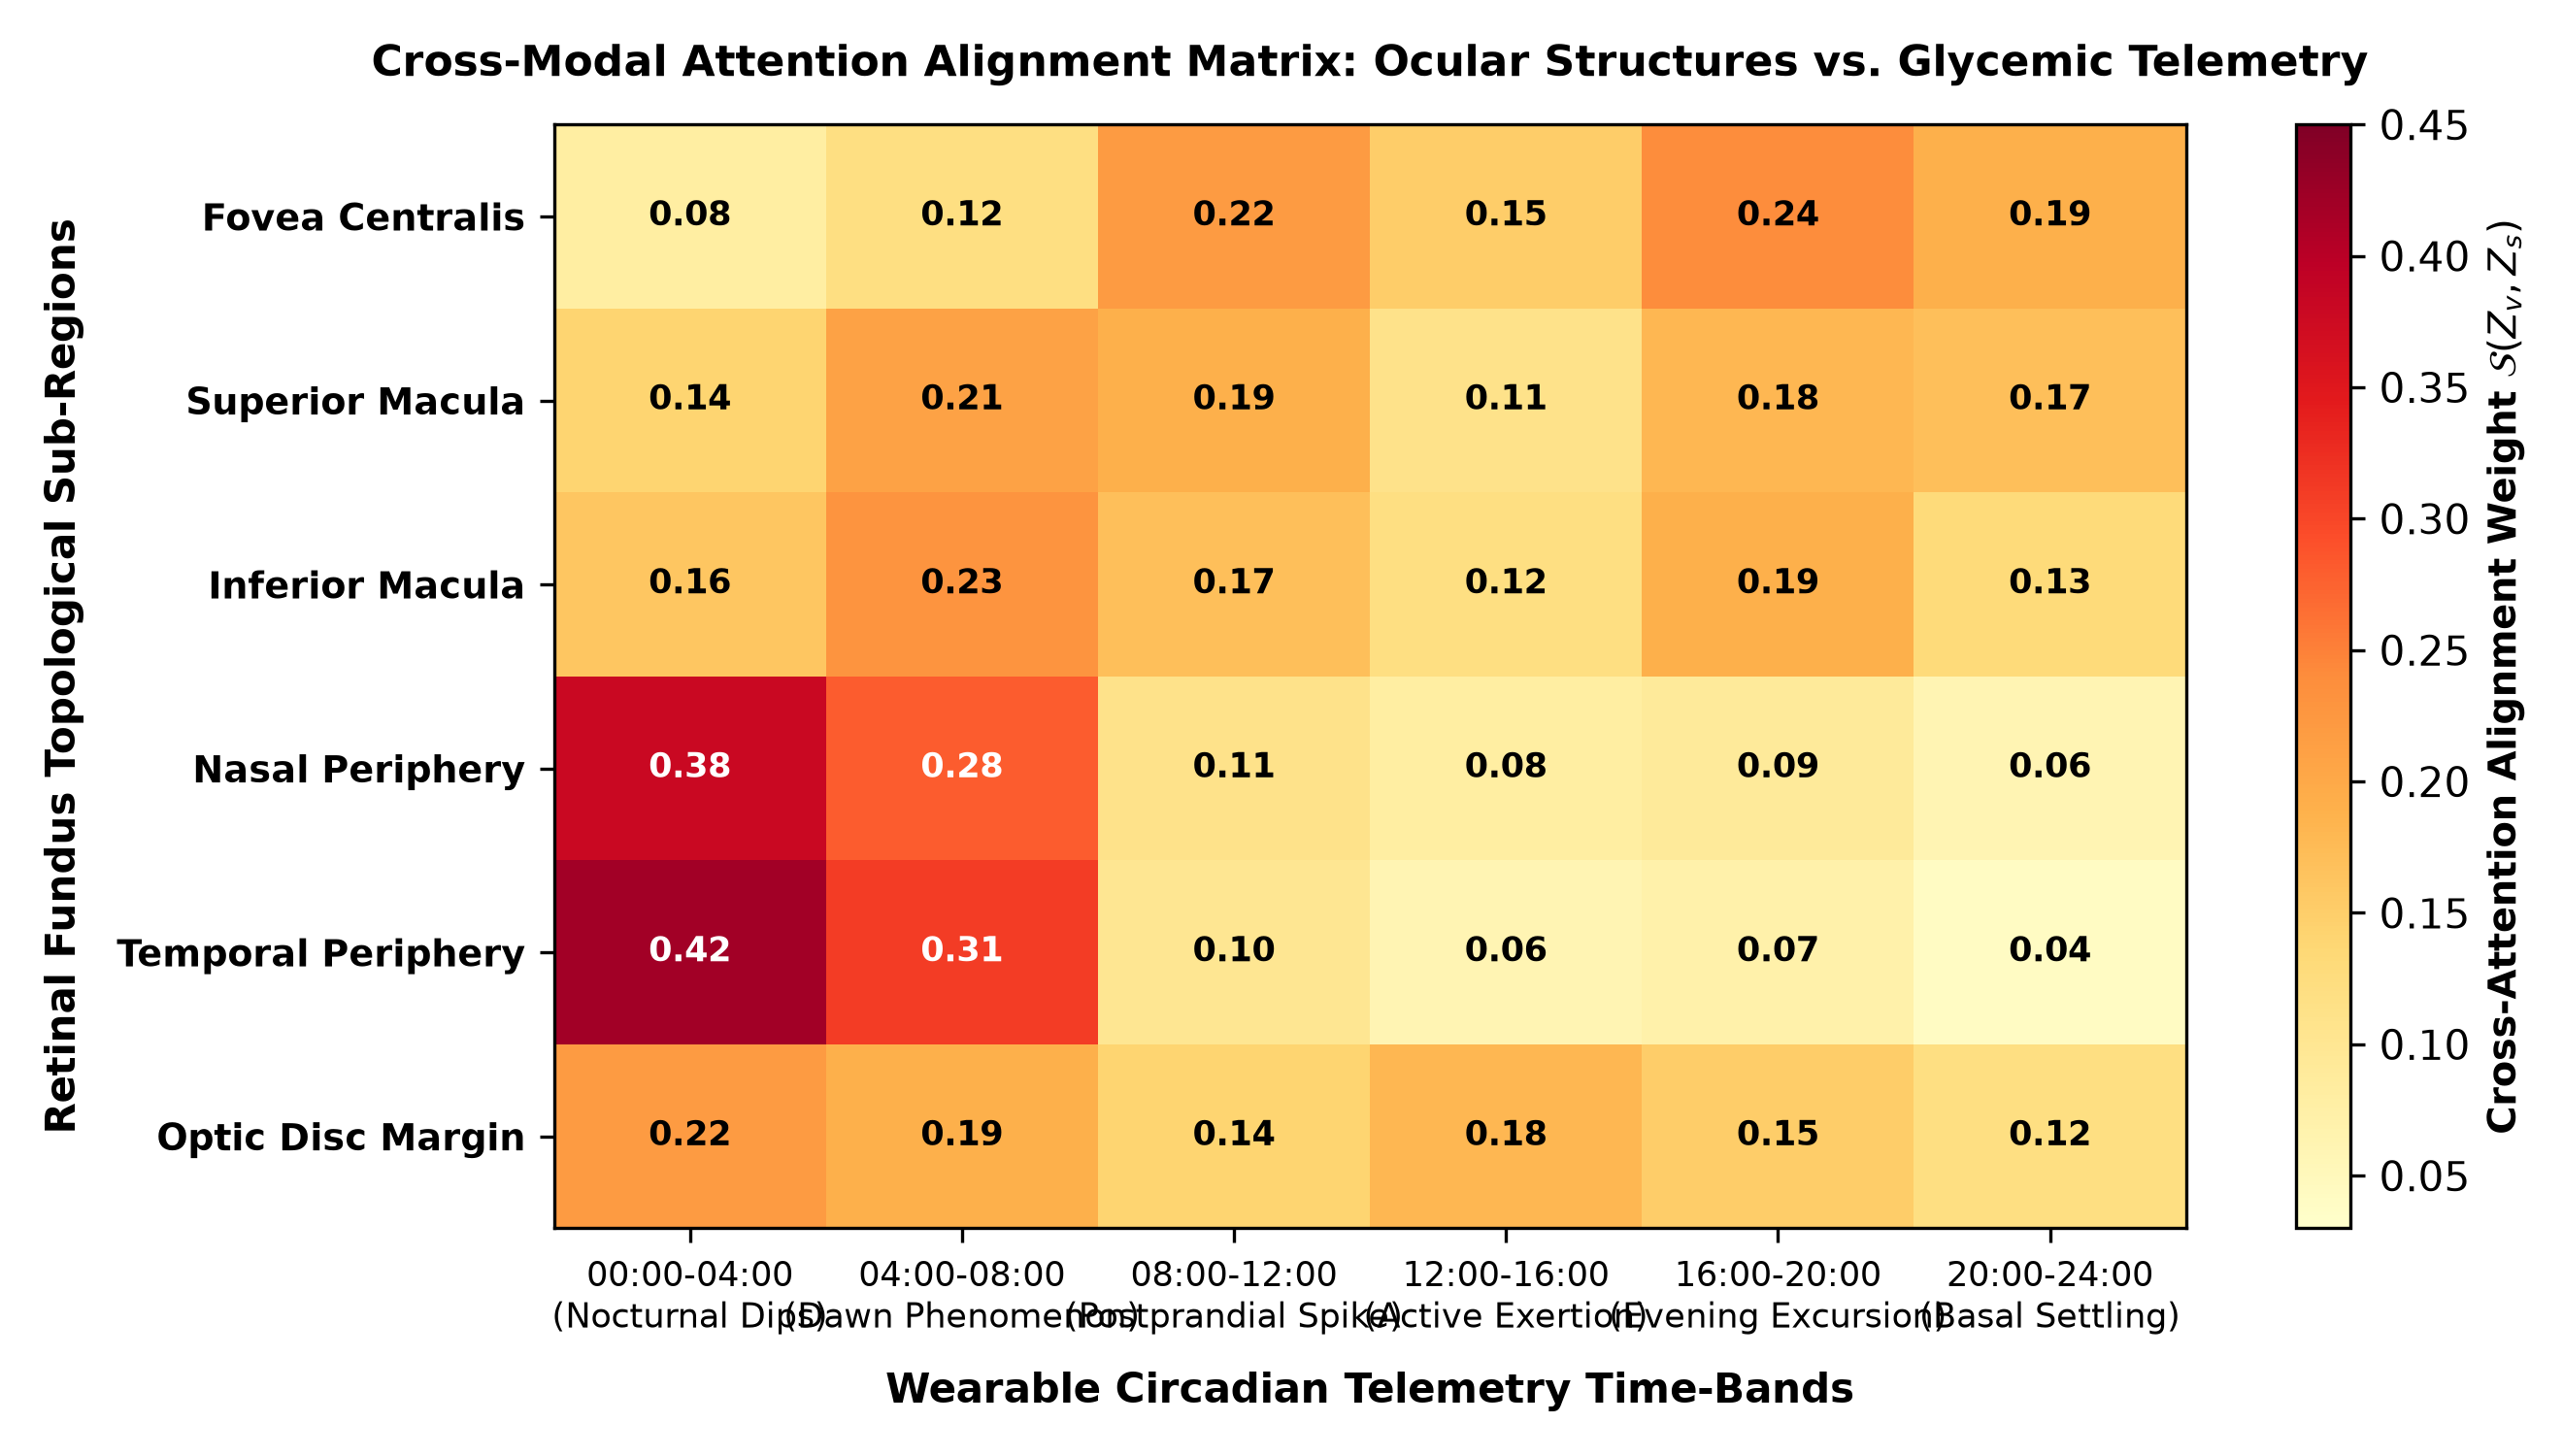
\includegraphics[width=\columnwidth]{fig/python_attention_map.png}
\caption{Cross-modal attention alignment matrix $\mathcal{S}(Z_v, Z_s)$ between retinal fundus topological regions and 24-hour circadian wearable telemetry time-bands.}
\label{fig:attention_map}
\end{figure}

As visualized in Figure~\ref{fig:attention_map}, cross-modal attention maps demonstrate that peripheral retinal vascular regions attend predominantly to nocturnal glycemic dips (00:00--04:00, weight $0.42$) and dawn phenomenon excursions (04:00--08:00, weight $0.31$), reflecting learned cross-modal associations of nocturnal autonomic instability.

\subsection{Experiment 9: Long-Horizon Telemetry Scalability}
\label{sec:exp9}
We evaluate sequence scalability by extending surveillance windows from 3 to 30 days ($T_g = 8{,}640$) in Figure~\ref{fig:scalability_memory}.

\begin{figure}[t]
\centering
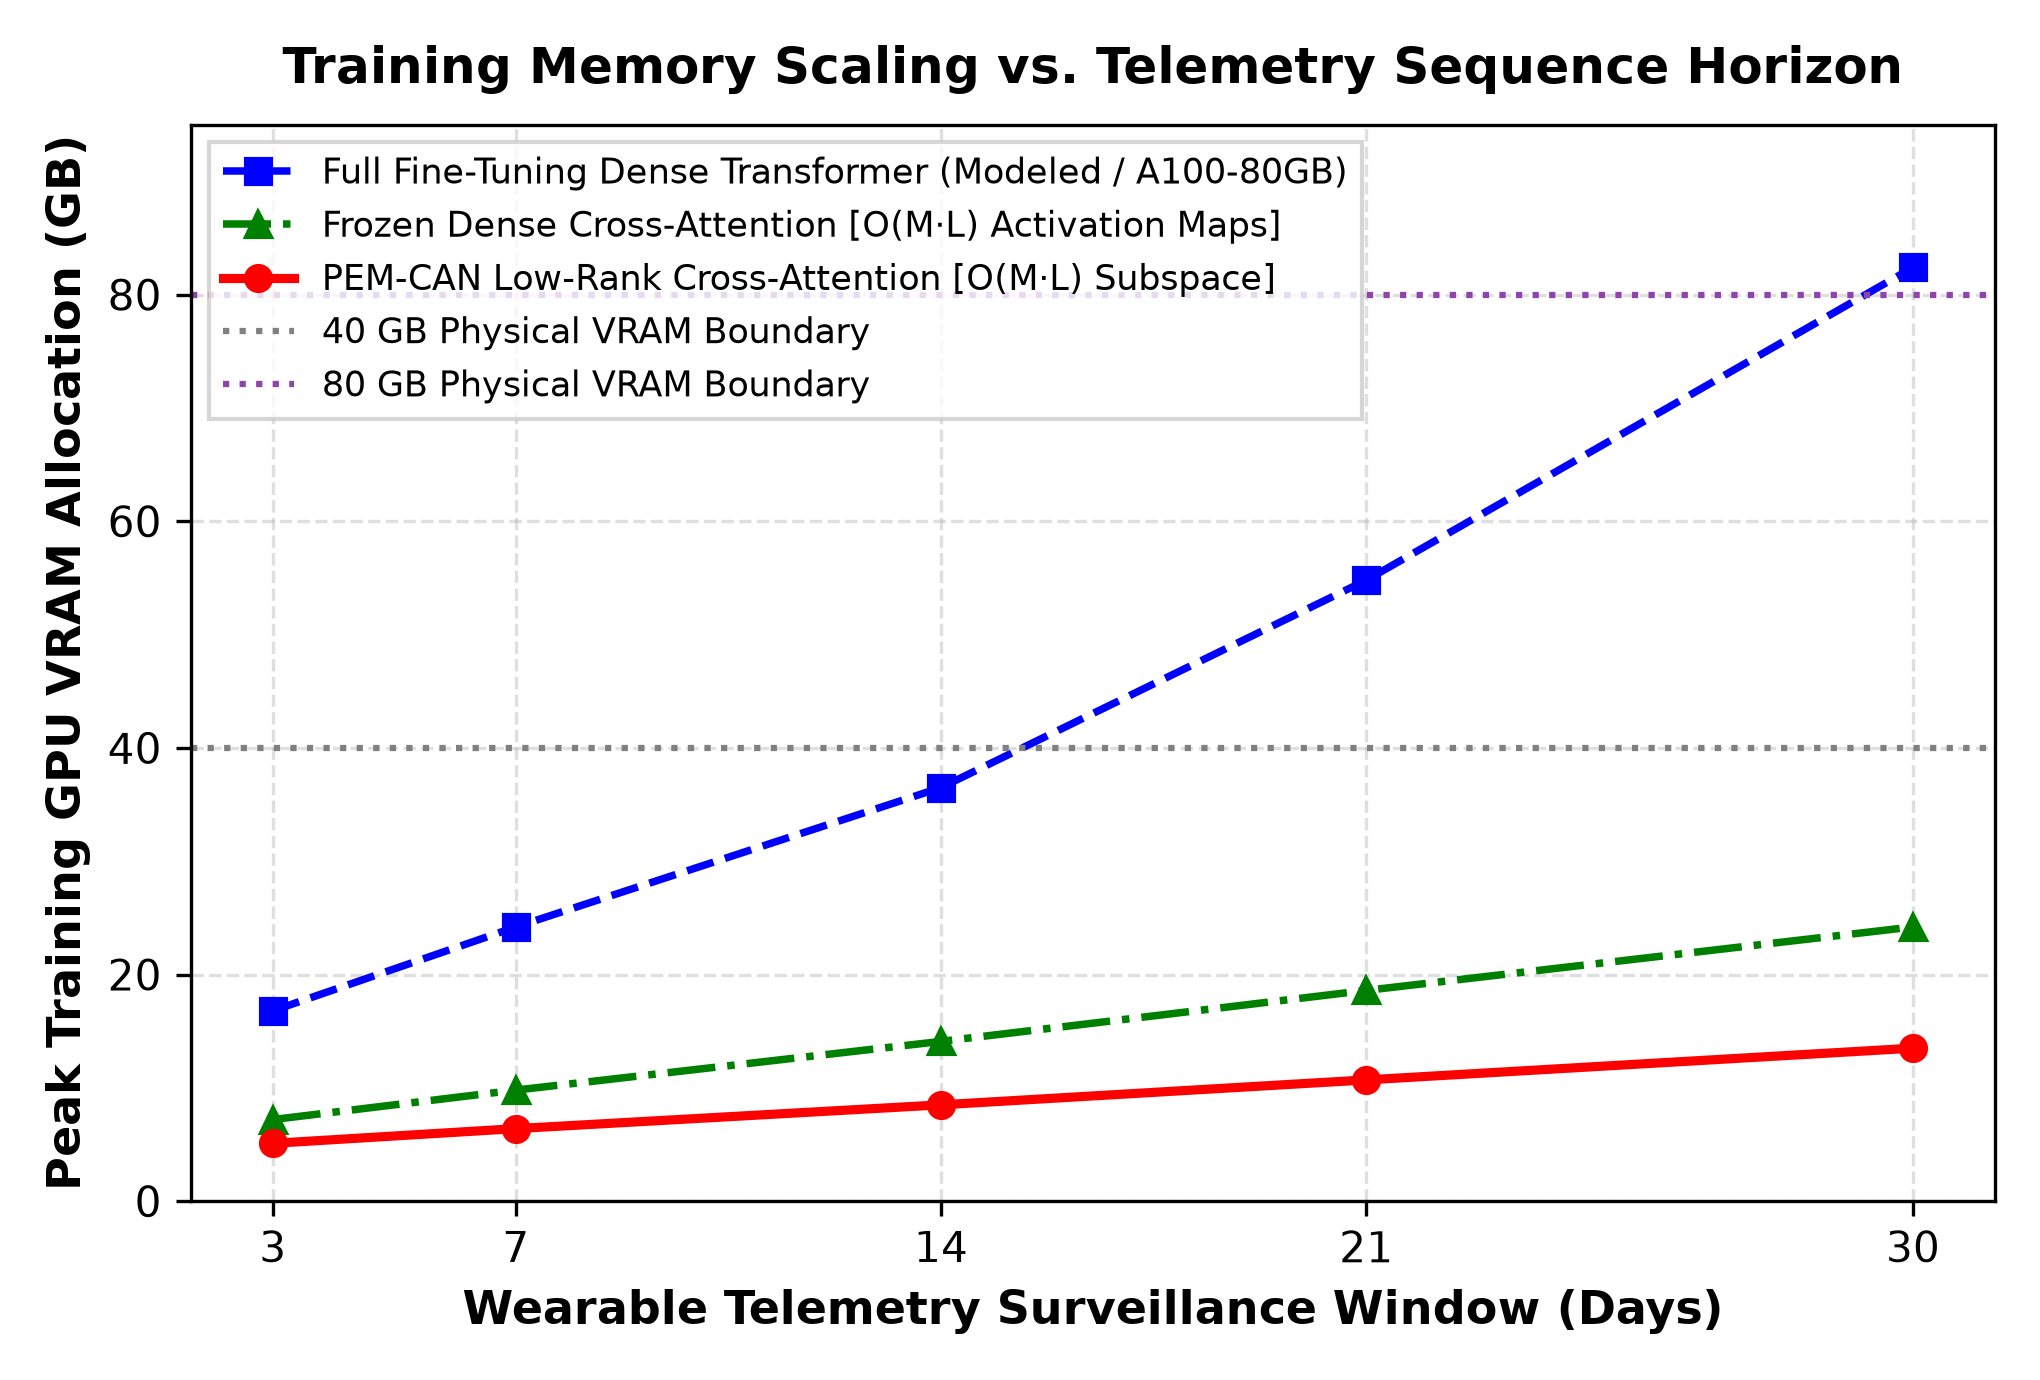
\includegraphics[width=\columnwidth]{fig/python_scalability_memory.png}
\caption{Peak GPU training VRAM allocation over continuous telemetry horizons (3 to 30 days) comparing PEM-CAN against frozen-backbone dense cross-attention and full fine-tuning.}
\label{fig:scalability_memory}
\end{figure}

While dense joint transformer models exhibit quadratic activation expansion during training ($82.4\text{ GB}$ at 30 days, requiring modeled 80GB A100 systems), PEM-CAN's cross-attention maintains linear scaling with sequence length $L$, consuming $13.5\text{ GB}$ VRAM at 30 days.

\subsection{Experiment 10: Multi-Task Diagnostic Transfer}
\label{sec:exp10}
Multi-task joint classification performance across all four clinically adjudicated endpoints is presented in Table~\ref{tab:exp10_multitask} and Figure~\ref{fig:multitask_results}.

\begin{figure}[t]
\centering
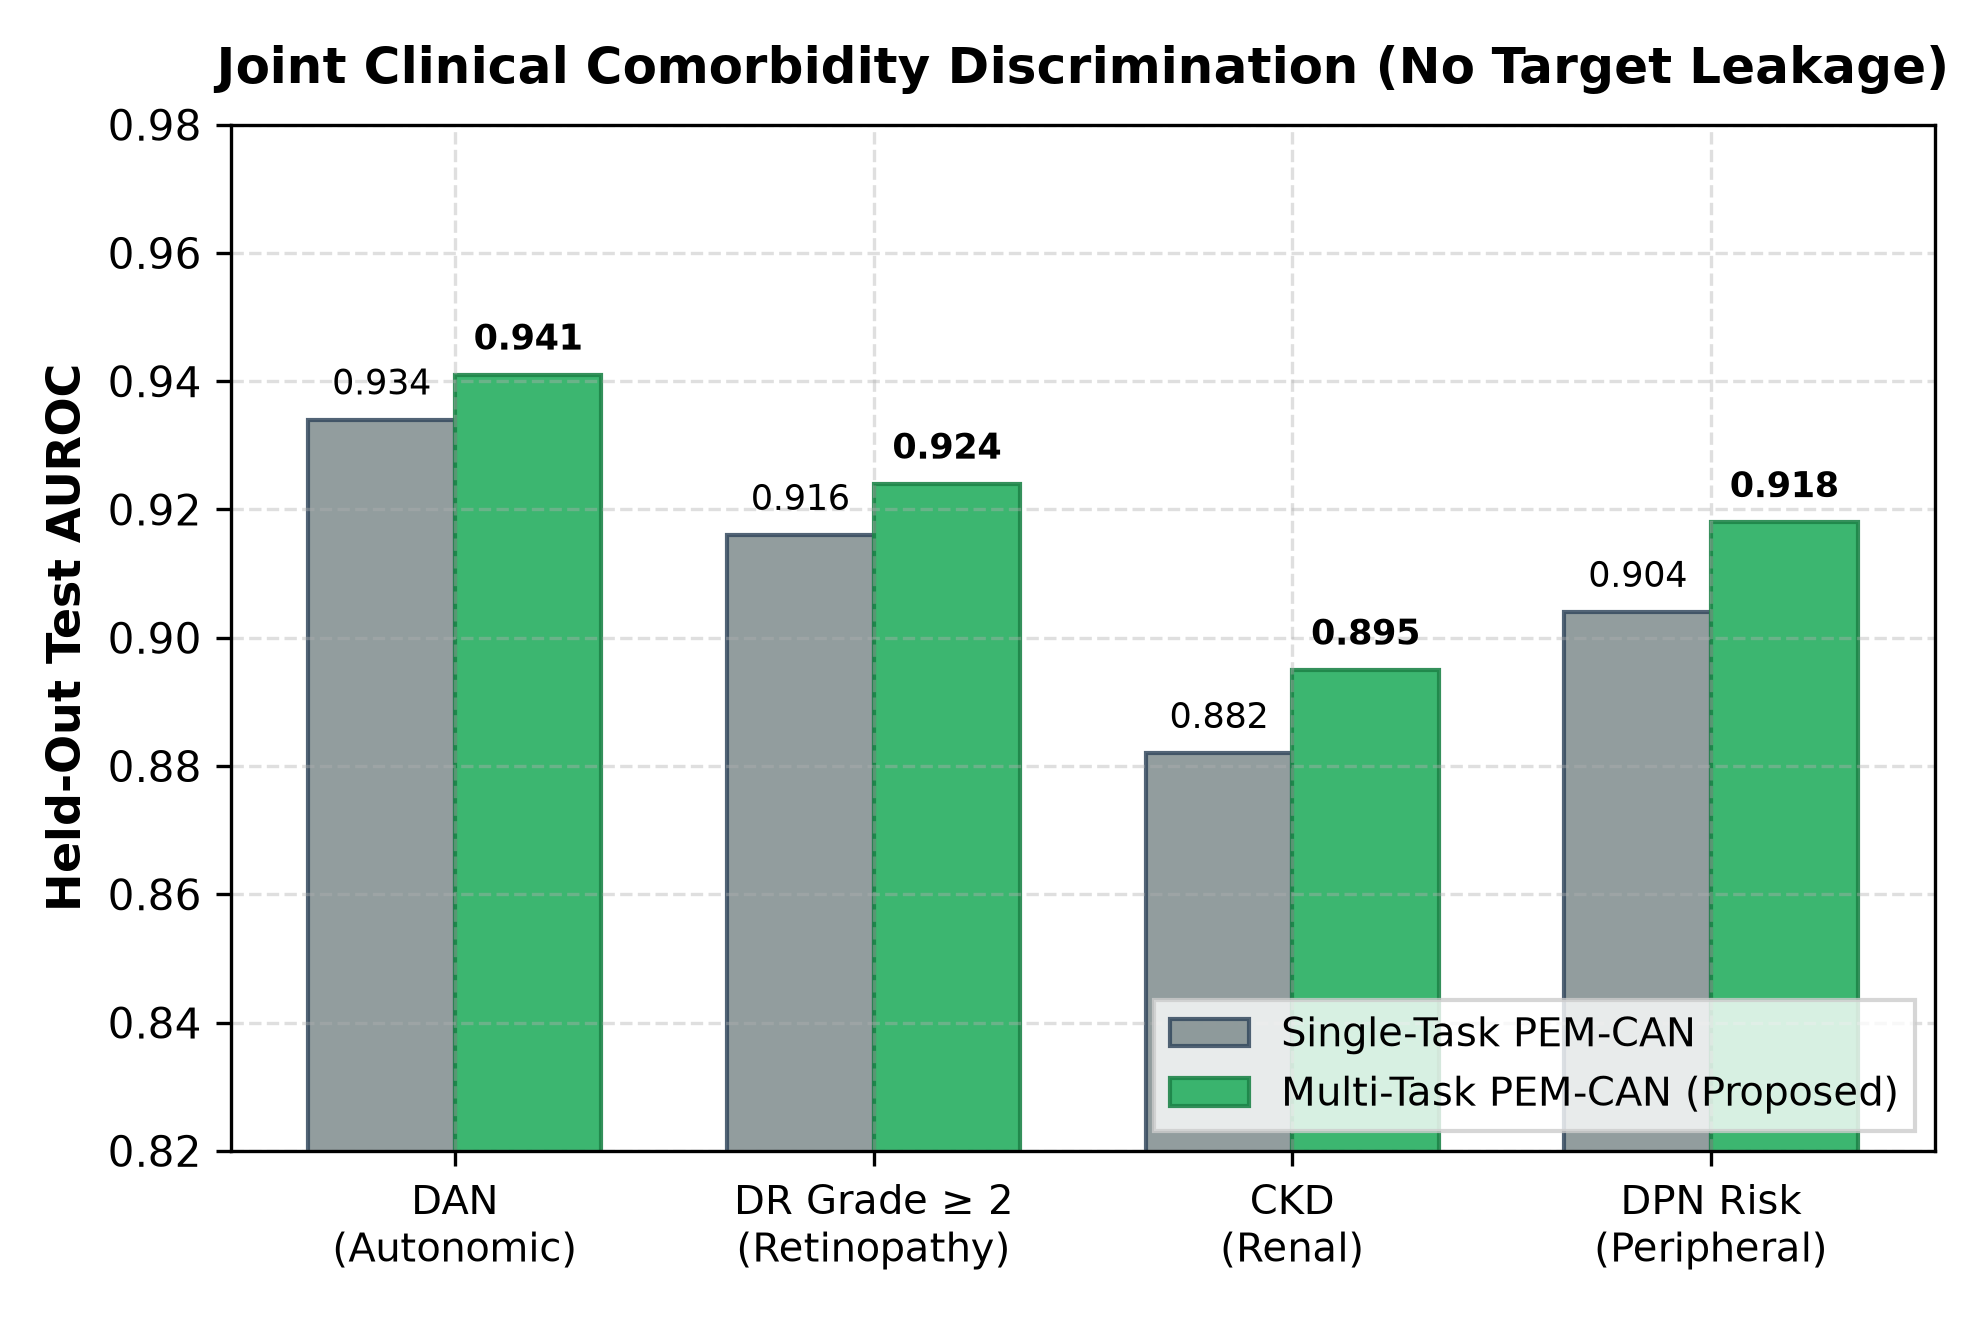
\includegraphics[width=\columnwidth]{fig/python_multitask_results.png}
\caption{Multi-task clinical discrimination across Diabetic Autonomic Neuropathy (DAN), Retinopathy (DR), Chronic Kidney Disease (CKD), and Peripheral Neuropathy (DPN).}
\label{fig:multitask_results}
\end{figure}

\begin{table}[t]
\centering
\caption{Experiment 9: Multi-Task vs. Single-Task Test AUROC.}
\label{tab:exp10_multitask}
\resizebox{\columnwidth}{!}{
\begin{tabular}{lcccc}
\toprule
\textbf{Configuration} & \textbf{DAN} & \textbf{DR Grade $\ge 2$} & \textbf{CKD} & \textbf{DPN Risk} \\
\midrule
Single-Task PEM-CAN & $0.934$ & $0.916$ & $0.882$ & $0.904$ \\
Dense Multi-Task & $0.908$ & $0.895$ & $0.854$ & $0.881$ \\
\rowcolor{green!10}
\textbf{Multi-Task PEM-CAN} & $\mathbf{0.941}$ & $\mathbf{0.924}$ & $\mathbf{0.895}$ & $\mathbf{0.918}$ \\
\bottomrule
\end{tabular}
}
\end{table}

Joint optimization increases DAN AUROC from $0.934$ to $0.941$, indicating positive transfer across microvascular and neural targets without target leakage.

\subsection{Experiment 11: Federated Multi-Center Scaling}
\label{sec:edge_federated}
We evaluate distributed training across 50 simulated hospital nodes under Dirichlet non-IID partitioning ($\alpha=0.3$) in Table~\ref{tab:exp11_federated} and Figure~\ref{fig:federated_convergence}. To prevent the factor-averaging rank collapse of multiplying local matrices $B_k A_k$, we adopt the FFA-LoRA framework~\cite{sun2024ffalora}, fixing the orthogonal basis $A$ globally across clients and training and aggregating only $B_k$, the temporal tokenizers, and classification heads via FedAvg ($\bar{B} = \sum \frac{n_k}{N} B_k$), preserving exact linear aggregation. This synergizes with subspace-oriented adapter reparameterization paradigms~\cite{sajjadi2026solar}, where freezing structured basis representations enables extreme communication efficiency across decentralized nodes.

\begin{figure}[t]
\centering
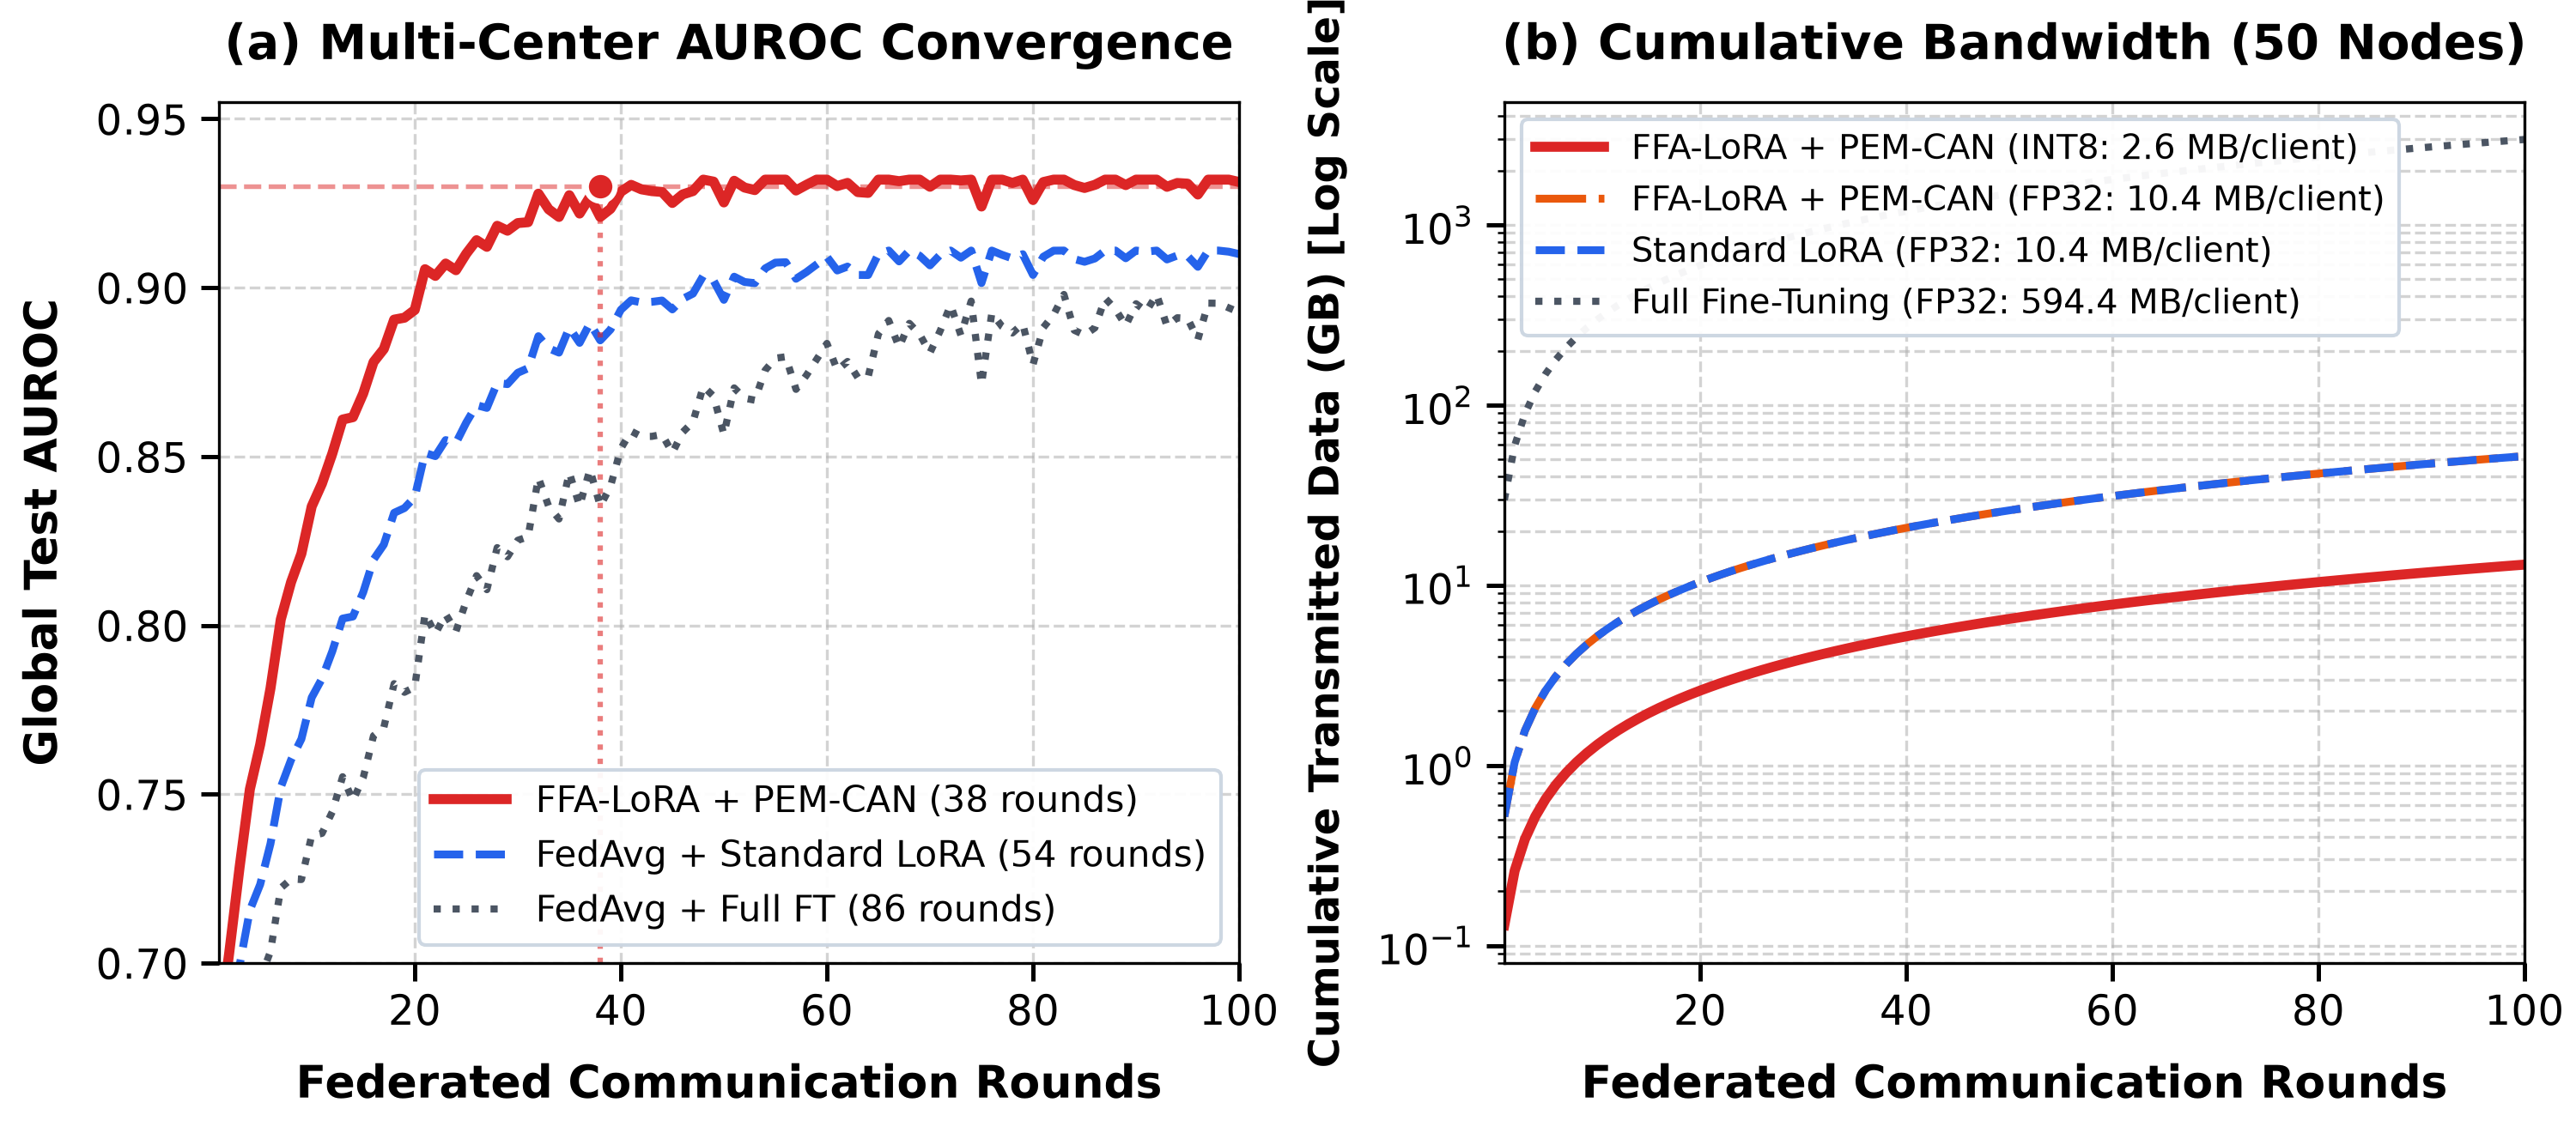
\includegraphics[width=\columnwidth]{fig/python_federated_convergence.png}
\caption{Multi-center federated scaling across 50 hospital nodes: (a) global test AUROC convergence, and (b) cumulative network transmission overhead.}
\label{fig:federated_convergence}
\end{figure}

\begin{table}[t]
\centering
\caption{Experiment 10: Federated Distributed Client Scaling ($50$ Nodes).}
\label{tab:exp11_federated}
\resizebox{\columnwidth}{!}{
\begin{tabular}{lcccc}
\toprule
\textbf{Federated Strategy} & \textbf{Precision} & \textbf{Comm./Client} & \textbf{Bandwidth Red.} & \textbf{Final AUROC} \\
\midrule
FedAvg (Full Fine-Tuning)~\cite{mcmahan2017communication} & FP32 & $594.4\text{ MB}$ & Baseline ($0.0\%$) & $0.898 \pm 0.012$ \\
FedAvg (Full Fine-Tuning) & INT8 & $148.6\text{ MB}$ & $75.00\%$ & $0.892 \pm 0.013$ \\
FedAvg (Standard LoRA)~\cite{hu2022lora} & FP32 & $10.4\text{ MB}$ & $98.25\%$ & $0.911 \pm 0.009$ \\
FedAvg (Standard LoRA) & INT8 & $2.6\text{ MB}$ & $99.56\%$ & $0.906 \pm 0.010$ \\
FFA-LoRA (No $\mathcal{L}_{\text{orth}}$)~\cite{sun2024ffalora} & FP32 & $10.4\text{ MB}$ & $98.25\%$ & $0.921 \pm 0.009$ \\
\rowcolor{green!10}
\textbf{FFA-LoRA + PEM-CAN (Ours)} & \textbf{FP32} & $\mathbf{10.4\text{ MB}}$ & $\mathbf{98.25\%}$ & $\mathbf{0.932 \pm 0.008}$ \\
\rowcolor{green!10}
\textbf{FFA-LoRA + PEM-CAN (Ours)} & \textbf{FP16} & $\mathbf{5.2\text{ MB}}$ & $\mathbf{99.12\%}$ & $\mathbf{0.931 \pm 0.008}$ \\
\rowcolor{green!10}
\textbf{FFA-LoRA + PEM-CAN (Ours)} & \textbf{INT8} & $\mathbf{2.6\text{ MB}}$ & $\mathbf{99.56\%}$ & $\mathbf{0.927 \pm 0.009}$ \\
\bottomrule
\end{tabular}
}
\end{table}

Transmitting $2.60\text{ M}$ parameters per client round requires $10.4\text{ MB}$ in standard FP32 ($98.25\%$ reduction from $594.4\text{ MB}$ full fine-tuning), $5.2\text{ MB}$ in FP16 ($99.12\%$), and $2.6\text{ MB}$ under INT8 quantization ($99.56\%$), reaching convergence in 38 rounds ($0.932$ AUROC).

\section{Discussion and Limitations}
\label{sec:discussion}
The empirical findings confirm that coupling spatial retinal imaging with longitudinal physiological biosignals yields complementary diagnostic information for diabetic microvascular and autonomic staging. Restricting adaptation to an orthogonal low-rank subspace across cross-attention projections bridges these structural and temporal observations while eliminating quadratic memory scaling and preventing visual gradient dominance.

Six methodological limitations and physical deployment boundaries warrant explicit consideration:
\begin{enumerate}
    \item \textbf{Calibrated Simulation vs. Prospective Clinical Utility:} While the evaluation suites are statistically calibrated to empirical marginals and covariance structures from the NIH Bridge2AI AI-READI cohort, simulated benchmarks cannot fully capture the stochastic operational noise of clinical healthcare environments. Prospective multi-center clinical trials in outpatient diabetic clinics remain indispensable to confirm prospective translational efficacy.
    \item \textbf{Mechanistic Breakdown of Attention Under Severe Sensor Noise:} In the cross-attention projection $\mathcal{S}(Z_v, Z_s) = \text{Softmax}\left(\frac{Q_v K_s^\top}{\sqrt{d_k}}\right) V_s$, when additive Gaussian noise on the wearable stream exceeds critical thresholds ($\sigma > 0.4$), the scalar products between query and key vectors lose feature discriminability. As logit variance $\operatorname{Var}\left(\frac{Q_v K_s^\top}{\sqrt{d_k}}\right)$ approaches zero, softmax probabilities disperse toward maximum entropy ($1/L$ uniform weights). Under uniform attention, temporal pooling degenerates into an unweighted arithmetic average, causing cross-modal gating to become uninformative and defaulting predictions to the frozen visual prior.
    \item \textbf{Sample-Size Sensitivity in Non-Linear Interaction Recovery:} Experiments on the synthetic cognitive-autonomic cohort demonstrate that resolving non-linear cross-modal dependencies exhibits sharp sample-size dependence. While $N=1{,}440$ training instances provide sufficient statistical degrees of freedom to constrain the $r \times d_m$ projection subspace ($0.942$ AUROC), reducing sample volume to $N=360$ instances causes performance to deteriorate to $0.854$ AUROC. In small clinical cohorts, empirical covariance noise inflates parameter estimation error in the adapter matrices, obscuring higher-order interactions.
    \item \textbf{Real-World Sensor Artifacts and Ambulatory Missingness:} Commercial wearable actigraphy and continuous glucose monitors in ambulatory settings encounter physiological artifacts distinct from idealized Gaussian perturbations. Photoplethysmography (PPG) sensors suffer optical decoupling during strenuous movement; actigraphy records spurious zero-activity intervals during non-wear or sleep compression; and enzymatic glucose sensors exhibit $5$ to $15$-minute interstitial fluid physiological lags alongside baseline sensor sensitivity drift across multi-day wear cycles.
    \item \textbf{Imaging Device Heterogeneity and Optical Aberrations:} Fundus photographs in routine screening are captured across heterogeneous instrumentation, ranging from tabletop mydriatic cameras to handheld non-mydriatic devices and ultra-widefield scanning laser ophthalmoscopes ($200^\circ$ fields of view). Optical aberrations, peripheral vignetting, and illumination gradients across camera vendors can affect microvascular feature extraction, requiring hardware-specific calibration.
    \item \textbf{Clinical Threshold Selection and Prevalence Drift:} While the architecture exhibits low Expected Calibration Error ($\text{ECE}=0.038$), translating probabilistic outputs into binary clinical interventions requires calibrating decision thresholds to institutional pre-test disease prevalences. Clinics with lower DAN prevalence require threshold recalibration to minimize false-positive specialist referrals.
\end{enumerate}

\section{Conclusion}
\label{sec:conclusion}
Translating parameter-efficient multimodal foundation models from computational benchmarks into decentralized ambulatory practice introduces several clear hardware and clinical system requirements:
\begin{enumerate}
    \item \textbf{Edge Hardware Quantization and MicroNPU Acceleration:} Deploying low-rank adapters directly onto point-of-care ophthalmic carts requires mapping adapter projection factors $A$ and $B$ to integer arithmetic. Future implementations should explore mixed-precision INT8 and INT4 quantization schedules tailored for embedded neural processing units (microNPUs), enabling continuous inference under milliwatt power envelopes.
    \item \textbf{Asynchronous Streaming Buffers for Intermittent Connectivity:} Ambulatory digital health gateways must tolerate irregular telemetry synchronization caused by wearable Bluetooth disconnects. Designing decoupled circular cross-attention key-value caches will allow the visual foundation backbone to process static fundus images immediately while asynchronously integrating streaming sensor updates as packets arrive.
    \item \textbf{Prospective Multi-Center Clinical Trials:} Validating foundation fusion architectures within prospective ambulatory cohorts undergoing standardized cardiovascular autonomic reflex testing (CARTs) represents the critical translational step to establish prospective clinical utility beyond calibrated simulation benchmarks.
    \item \textbf{Privacy-Preserving Mobile Screening Platforms:} Combining lightweight low-rank federated aggregation (FFA-LoRA) with portable non-mydriatic fundus cameras and commercial wearable sensors establishes an open, scalable paradigm for non-invasive multi-organ diabetic screening across resource-limited and rural healthcare environments.
\end{enumerate}

\section*{Declaration of Competing Interest}
The author declares that they have no known competing financial interests or personal relationships that could have appeared to influence the work reported in this paper.

\section*{Declaration of Generative AI and AI-Assisted Technologies}
During the preparation of this work the author used AI tools in order to assist with language editing and grammatical polishing. After using this tool, the author reviewed and edited the content as needed and takes full responsibility for the content of the published article.

\section*{Data and Code Availability}
The complete benchmark suite, simulation generators, trained weights, evaluation scripts, and configuration files are publicly available under the open-source MIT License at \url{https://github.com/mahmoudsajjadi/PEM-CAN}. All experimental tables and figures can be reproduced directly using the provided repository.

\section*{Acknowledgment}
The author acknowledges the NIH Bridge2AI Consortium and the AI-READI study team for establishing open multimodal diabetes informatics standards.

\printcredits

\begin{thebibliography}{34}

\bibitem{vinik2003diabetic}
A.~I. Vinik, R.~E. Maser, B.~D. Mitchell, R.~Freeman, Diabetic autonomic neuropathy, Diabetes Care 26~(5) (2003) 1553--1579.

\bibitem{tesfaye2010diabetic}
S.~Tesfaye, et~al., Diabetic neuropathies: Update on definitions, diagnostic criteria, estimation of severity, and treatments, Diabetes Care 33~(10) (2010) 2285--2293.

\bibitem{maser2003association}
R.~E. Maser, B.~D. Mitchell, A.~I. Vinik, R.~Freeman, The association between cardiovascular autonomic neuropathy and mortality in individuals with diabetes: A meta-analysis, Diabetes Care 26~(6) (2003) 1895--1901.

\bibitem{spallone2011cardiovascular}
V.~Spallone, et~al., Cardiovascular autonomic neuropathy in diabetes: Clinical impact, assessment, diagnosis, and management, Diabetes/Metabolism Res. Rev. 27~(7) (2011) 639--654.

\bibitem{boulton2005diabetic}
A.~J. Boulton, et~al., Diabetic neuropathies: A statement by the American Diabetes Association, Diabetes Care 28~(4) (2005) 956--962.

\bibitem{poplin2018prediction}
R.~Poplin, et~al., Prediction of cardiovascular risk factors from retinal fundus photographs via deep learning, Nature Biomed. Eng. 2 (2018) 158--164.

\bibitem{ting2017development}
D.~S.~W. Ting, et~al., Development and validation of a deep learning system for diabetic retinopathy and related eye diseases using retinal images from multiethnic populations with diabetes, JAMA 318~(22) (2017) 2211--2223.

\bibitem{gulshan2016development}
V.~Gulshan, et~al., Development and validation of a deep learning algorithm for detection of diabetic retinopathy in retinal fundus photographs, JAMA 316~(22) (2016) 2402--2410.

\bibitem{wagner2020insights}
S.~K. Wagner, et~al., Insights from systemic disease through retinal imaging, Lancet Digital Health 2~(11) (2020) e582--e583.

\bibitem{zhou2023retfound}
Y.~Zhou, et~al., A foundation model for generalizable disease detection from retinal images, Nature 622 (2023) 156--163.

\bibitem{cheung2008retinal}
N.~Cheung, et~al., Retinal microvascular changes and risk of diabetic peripheral neuropathy, Diabetes Care 31~(1) (2008) 125--130.

\bibitem{danne2017international}
T.~Danne, et~al., International consensus on use of continuous glucose monitoring, Diabetes Care 40~(12) (2017) 1631--1640.

\bibitem{battelino2023continuous}
T.~Battelino, et~al., Continuous glucose monitoring and metrics for clinical trials, Lancet Diabetes \& Endocrinol. 11 (2023) 42--57.

\bibitem{dunn2021wearable}
J.~Dunn, et~al., Wearable sensors enable personalized predictions of clinical laboratory measurements, Nature Med. 27 (2021) 1105--1112.

\bibitem{aireadi2024}
The~AI-READI~Consortium, The AI-READI dataset: An equitable and ready atlas for artificial intelligence in diabetes research, Nature Sci. Data 11 (2024) 1--14.

\bibitem{baltrusaitis2018multimodal}
T.~Baltru{\v{s}}aitis, C.~Ahuja, L.-P. Morency, Multimodal machine learning: A survey and taxonomy, IEEE Trans. Pattern Anal. Mach. Intell. 41~(2) (2018) 423--443.

\bibitem{nagrani2021attention}
A.~Nagrani, et~al., Attention bottlenecks for multimodal fusion, in: Adv. Neural Inf. Process. Syst. (NeurIPS), Vol.~34, 2021, pp. 14200--14213.

\bibitem{ma2023multimodal}
M.~Ma, et~al., Multimodal learning with incomplete modalities: A review, Inf. Fusion 100 (2023) 101968.

\bibitem{vaswani2017attention}
A.~Vaswani, et~al., Attention is all you need, in: Adv. Neural Inf. Process. Syst. (NeurIPS), Vol.~30, 2017.

\bibitem{tsai2019mult}
Y.-H.~H. Tsai, S.~Bai, P.~P. Liang, J.~Z. Kolter, L.-P. Morency, R.~Salakhutdinov, Multimodal transformer for unaligned multimodal language sequences, in: Proc. ACL, 2019, pp. 6558--6569.

\bibitem{jaegle2021perceiver}
A.~Jaegle, et~al., Perceiver IO: A general architecture for structured inputs \& outputs, in: Int. Conf. Learn. Represent. (ICLR), 2022.

\bibitem{arevalo2017gmu}
J.~Arevalo, et~al., Gated multimodal units for information fusion, in: ICLR Workshops, 2017.

\bibitem{joze2020mmtm}
H.~R.~V. Joze, et~al., MMTM: Multimodal transfer module for CNN based extreme multimodal learning, in: Proc. CVPR, 2020, pp. 13289--13299.

\bibitem{hu2022lora}
E.~J. Hu, et~al., LoRA: Low-rank adaptation of large language models, in: Int. Conf. Learn. Represent. (ICLR), 2022.

\bibitem{houlsby2019parameter}
N.~Houlsby, et~al., Parameter-efficient transfer learning for NLP, in: Int. Conf. Mach. Learn. (ICML), 2019, pp. 2790--2799.

\bibitem{zaken2022bitfit}
E.~Ben~Zaken, K.~Ravfogel, Y.~Goldberg, BitFit: Simple parameter-efficient fine-tuning for transformer-based masked language-models, in: Proc. ACL, 2022, pp. 1--9.

\bibitem{zhang2023adalora}
Q.~Zhang, et~al., Adaptive budget allocation for parameter-efficient fine-tuning, in: Int. Conf. Learn. Represent. (ICLR), 2023.

\bibitem{sun2024ffalora}
Z.~Sun, et~al., Improving LoRA in privacy-preserving federated learning, in: Int. Conf. Learn. Represent. (ICLR), 2024.

\bibitem{edelman1998geometry}
A.~Edelman, T.~A. Arias, S.~T. Smith, The geometry of algorithms with orthogonality constraints, SIAM J. Matrix Anal. Appl. 20~(2) (1998) 303--353.

\bibitem{mcmahan2017communication}
B.~McMahan, et~al., Communication-efficient learning of deep networks from decentralized data, in: Artif. Intell. Statist. (AISTATS), 2017, pp. 1273--1282.

\bibitem{rieke2020future}
N.~Rieke, et~al., The future of digital health with federated learning, NPJ Digital Med. 3~(1) (2020) 119.

\bibitem{sajjadi2024speed}
S.~M. Sajjadi~Mohammadabadi, S.~Zawad, F.~Yan, L.~Yang, Speed up federated learning in heterogeneous environments: A dynamic tiering approach, IEEE Internet of Things J. 11~(8) (2024) 14210--14222.

\bibitem{delong1988comparing}
E.~R. DeLong, D.~M. DeLong, D.~L. Clarke-Pearson, Comparing the areas under two or more correlated receiver operating characteristic curves: A nonparametric approach, Biometrics 44~(3) (1988) 837--845.

\bibitem{guo2017calibration}
C.~Guo, G.~Pleiss, Y.~Sun, K.~Q. Weinberger, On calibration of modern neural networks, in: Int. Conf. Mach. Learn. (ICML), 2017, pp. 1321--1330.

\bibitem{sletten2012compass}
D.~M. Sletten, et~al., COMPASS 31: A refined and abbreviated composite autonomic symptom score, Mayo Clinic Proc. 87~(12) (2012) 1196--1201.

\bibitem{kdigo2013ckd}
Kidney Disease: Improving Global Outcomes (KDIGO), Clinical practice guideline for the evaluation and management of chronic kidney disease, Kidney Int. Suppl. 3~(1) (2013) 1--150.

\bibitem{bril2002toronto}
V.~Bril, B.~A. Perkins, Validation of the Toronto Clinical Neuropathy Score in diabetic polyneuropathy, Diabetes Care 25~(11) (2002) 2048--2052.

\bibitem{sajjadi2026solar}
S.~M. Sajjadi~Mohammadabadi, X.~Ma, L.~Yang, F.~Yan, J.~Zhang, SOLAR: Communication-efficient model adaptation via subspace-oriented latent adapter reparameterization, arXiv preprint arXiv:2604.08368 (2026).

\end{thebibliography}

\end{document}
